\documentclass[parskip=full]{scrartcl}
\usepackage[utf8]{inputenc}
\usepackage[T1]{fontenc}
\usepackage[ngerman]{babel}
\usepackage{hyperref}
\usepackage{enumitem}
\usepackage{glossaries}
\usepackage{graphicx}

\usepackage[binary-units=true]{siunitx}
  \usepackage[autostyle=true,german=quotes]{csquotes}
\makeglossaries
%für die Nummerierung der Listen
\newcommand{\swtLabel}[1]{\textbf{/#1\arabic*0/}}

\newglossaryentry{PSE}{name=PSE,
                        description={Im PSE (Praxis der Softwareentwicklung)
                        lernen die Teilnehmer, ein vollständiges Softwareprojekt nach dem Stand der
                        Softwaretechnik in einem Team mit 5 bis 6 Teilnehmern
                        durchzuführen. Ziel ist es insbesondere, Verfahren des
                        Software-Entwurfs und der Qualitätssicherung praktisch
                        einzusetzen, Implementierungskompetenz umzusetzen, und
                        arbeitsteilig im Team zu kooperieren.}}
                      
\newglossaryentry{Lerngruppe}{name=Lerngruppe,
description={Eine Lerngruppe ist ein Zusammenschluss von Studierenden, welche
gemeinsam eine Bewertung abgeben für die \glspl{Projekt}inteilung. Zusätzlich
werden sie bei der Einteilung gesondert berücksichtigt, sodass Studierende einer
Lerngruppe möglichst ein Team bilden oder als Gruppe einem Team angehören.
}, plural=Lerngruppen}
\newglossaryentry{Guetekriterium}{name=Gütekriterium,
plural=Gütekriterien,description={Gütekriterien sind Kriterien, welche die Güte
einer Einteilung bestimmen. Anhand von Gütekriterien kann ein Vergleich und eine
Bewertung von Einteilungen vorgenommen werden. 
}}
\newglossaryentry{Projekt}{name=Projekt,
plural=Projekte, description={Ein Projekt ist ein zielgerichtetes Vorhaben,
welches von mindestens einem Team bearbeitet wird. Dieses Vorhaben wird von mehreren Projektbetreuern begleitet und unterstützt.
}}
\newglossaryentry{Projektbetreuer}{name=Projektbetreuer,
plural=Projektbetreuer, description={Ein Projektbetreuer ist eine Person, welche administrative und unterstützende Tätigkeiten eines oder mehrerer \glspl{Projekt} ausführt. Dabei kann ein Projektbetreuer mehrere Teams betreuen.
}}
\newglossaryentry{Admin}{name=Administrator,
plural=Administratoren, description={Ein Administrator ist eine Person, welche das PSE administrativ unterstützt und das Produkt konfiguriert.
}}
\newglossaryentry{Studierender}{name=Studierender,
plural=Studierende, description={Ein Studierender ist eine Person, welche eingeschrieben ist an einer Universität. In diesem Kontext sind nur Studierende gemeint, welche sich für das PSE angemeldet haben und an diesem teilnehmen wollen.
}}
\newglossaryentry{Team}{name=Team,
plural=Teams, description={Ein Team ist ein Zusammenschluss von Studierenden, welche gemeinsam ein Projekt bearbeiten.
}}
\newglossaryentry{SPO}{name=SPO,
plural=SPOs, description={Die SPO (Studienprüfungsordnung) regelt den Studienablauf, die Prüfungen und den Abschluss des Studiums.
}}
\newglossaryentry{Teilleistung}{name=bestandene Teilleistung, %bestandene weglassen?!
plural=bestandene Teilleistungen, description={Eine Teilleistung ist eine von den \glspl{Studierender}n zu erbringende Leistung, meist in Form einer schriftlichen Prüfung. Das bestehen einer oder mehrerer Teilleistungen führt zum bestehen eines \gls{Modul}s. Dies wird in der \gls{SPO} spezifiziert.
}}
\newglossaryentry{Modul}{name=Modul,
plural=Module, description={Ein Modul ist ein Zusammenschluss verschiedener Teilleistungen, welche das gleiche Thema abdecken. 
}}
\newglossaryentry{happyness}{name=Studierenden-Happyness,
plural=Studierenden-Happyness, description={Die Studierenden-Happyness ist ein
\gls{Guetekriterium} welches sich aus der  }} %TODO formulierung
\newglossaryentry{gesplitteteGruppe}{name=Anzahl der gesplittelen Lerngruppen,
 description={ Die Anzahl der gesplittelen Lerngruppen ist ein
 \gls{Guetekriterium} welches angiebt, wieviele Lerngruppen bei der Einteilung
 auseinander gerissen wurden}}

\newglossaryentry{nichtZugeteilt}{name=Anzahl der nicht Zugeteilten,
 description={Die Anzahl der nicht Zugeteilten ist ein 
\gls{Guetekriterium} welches angiebt, wie viele Studierende bei einer einteilung
nicht zugeteilt wurden }}

\begin{document}

\title{\textbf{STRAPSE}\\
        \large Supter Team Allocationt for PSE}

\author{D. Biester, E. Dohse, P. Faller, P. Loth, L. Seufert, S. Kopmann}
        
\maketitle
 
\pagebreak
\tableofcontents
\pagebreak

\section{Zielbestimmung}

Die Einteilung zu den Projektgruppen für das Modul \gls{PSE} wurde bisher über die Software \enquote{Webinscribe} gelöst.
\enquote{Webinscribe} ist dazu entworfen worden, Studierende zu Tutorien einzuteilen.
Zwar ähneln die Anforderungen an die PSE-Teameinteilung denen, der Tutoriumseinteilung,
jedoch sind sie nicht absolut deckungsgleich. 
Dadurch ist die aktuelle Lösung mit Webinscribe umständlich in der Bedienung und lässt Wünsche bezüglich hilfreicher Features offen.
So müssen beispielsweise die angebotenen Themen als Tutorien eingetragen werden. 
Oder eine manuelle Änderung der Einteilung ist nicht über eine Eingabemaske möglich.

Dem tritt unser Produkt entgegen.
Da es speziell auf die Bedürfnisse der PSE-Einteilung zugeschnitten ist, 
kann es eine konsistente und bequeme Benutzerschnittstelle anbieten.
Es löst das Problem, die Studierenden auf die angebotenen Projekte zu verteilen und kann dabei über die Eingabe von Parametern leicht konfiguriert werden.
Durch zusätzlich angebotene Features, wie die Verwaltung der Themen durch die Projektleiter selbst 
oder die Möglichkeit zur automatischen Benachrichtigung der betroffenen Studierenden und Betreuer über die
Einteilung, soll der Administrationsaufwand drastisch reduziert werden. 

Insgesamt entsteht dadurch für alle Beteiligten ein effektiver und smarter Workflow.


\subsection{Musskriterien}
 \begin{enumerate}[label=\swtLabel{M}]
   \item Datenerfassung: Studierende sollen auf einer Internetseite:   
   \begin{itemize}
     \item ihre Daten (siehe \ref{SDatenAnfang} bis \ref{SDatenEnde}),     
     \item ihre Projektvorlieben, 
     \item ihre \glspl{Teilleistung},
     \item und gegebenenfalls ihre \glspl{Lerngruppe}
   \end{itemize}
   in das Produkt eingeben können.
   \item Studierende können sich ?? %TODO Authenntifizierung formulieren
   \item Studierende können vor der Einteilung Lerngruppen erstellen, beitreten
    und diese wieder verlassen
    \item Verwaltung von Lerngruppen durch Studierende % Geneauer in FAs oder
    % auch schon hier?
   \item Das Produkt teilt nach folgenden Kriterien Studierenden Teams zu:
   \label{Mzuteilung}
   \begin{itemize}
     \item Wer die Voraussetzungen nicht erfüllt wird nicht eingeteilt
     \item Lerngruppen sollten zusammenbleiben
     \item Präferenzen der Studierenden werden berücksichtigt
   \end{itemize}
     \item Konfiguration der Einteilungskriterien möglich
   \item Manuelles Nachjustieren der Einteilung
   \item Berechnung von \glspl{Guetekriterium}
   \item Im- und Export der Studierendendaten und
   Einteilungen %TODO: formulierung 
   \item Möglichkeit des sukzessiven Eintragens von \glspl{Projekt}n
  
 \end{enumerate}


\subsection{Wunschkriterien}
\begin{enumerate}[label=\swtLabel{W}]
  \item Abbrechen der Berechnung der Zuteilung möglich 
    
    \item Wunschkriterien zur Lösung des Problems der Einteilung (\ref{Mzuteilung}):
    \begin{itemize}
        \item Eher 5er"=Teams als 6er"=Teams
        \item Teams möglichst mit Studierende im gleichen Fachsemester 
        \item Studierende bevorzugen, die bereits mehr Teilleistungen aus dem
        ersten Jahr bestanden haben.
    \end{itemize}    
    \item Authentifizierung via Shibboleth
    \item Benachrichtigung der Studierenden und Mitarbeiter über die Einteilung
    \item Verwaltung mehrerer Einteilungsergebnisse
    \item Möglichkeit der Verwaltung der \glspl{Projekt} durch die Betreuer  %TODO:
    % formulierung
    \item Nachjustierbarkeit bei Änderungen der SPO %TODO: überlegen ob
    % Pflichtkriterium: mehrere SPOs verwalten.
    \item Verwaltung über mehrere Semester hinweg
    \item Anzeige der Projektdetails für Studierende
    \item Stapelverarbeitung zur Berechnungen verschiedener Einteilungen mit
    unterschiedlichen Konfigurationen
    \item Verifikation der Studierenden-E-Mail-Adresse über einen
    Verifikationslink der an die, von Studierenden angegebenne E-Mail-Adresse
    geschickt wird
    \item Datenabgleich mit dem Campus Management System %TODO:
    % detail csv?
    \item Mobile Version der Webseite zur Nutzung auf Smartphones und Tabets
    
    
    
\end{enumerate}

\subsection{Abgrenzungskriterien}
\begin{enumerate}[label=\swtLabel{AG}]
 
  \item Das Produkt ist nicht für die Nutzung außerhalb des KITs bestimmt %Please dont do the Deppenapostroph!

\item Die Einteilungsfunktion ist nur für die Einteilung zum PSE, nicht
für die Vergabe sonstiger Praktikums- oder Tutoriumsplätze bestimmt
  
\end{enumerate}
\section{Produkteinsatz}
%Wissenschaftliche Mitarbeiter sollen durch das Produkt die Verwaltung der Pro-
%jekte und die Einteilung zur Praxis der Softwareentwicklung rechnerunterstützt
% durch-
%zuführen können.
%TODO formulierung
Das Produkt dient zum Einpflegen von \glspl{Projekt}n und zur Zuteilung von
Studierenden zu diesen \glspl{Projekt}n. Hierbei werden die Projektpräferenzen der
Studierenden berücksichtigt.


\subsection{Anwendungsbereiche}

\begin{itemize} 
  \item Projektverwaltung und "-zuteilung (universitärer Bereich) %TODO Detail
\end{itemize}

\subsection{Zielgruppe}
\begin{itemize} 
  \item \glspl{Studierender}
  \item \gls{Projektbetreuer}
  \item \gls{Admin}
\end{itemize}

\subsection{Betriebsbedingungen}
\begin{itemize} 
  \item Zugriff über eine Webseite
\end{itemize}
\section{Produktumgebung}

\begin{itemize} 
  \item Das Produkt läuft auf einem für alle Benutzer erreichbaren Webserver
\end{itemize}
\subsection{Server-Software}
\begin{itemize} 
  \item Apache"=Webserver (\texttt{HTTP, SMTP})
  \item MySQL"=Server
  \item ILP"=Solver Gurobi %TODO lizens
\end{itemize}
\subsection{Server-Hardware}
Mindestens:
\begin{itemize} 
  \item $\SI{16}{\giga\byte}$ Ram
  \item Intel i7 Quadcore mit 4 weiteren virtuellen Kernen 
  %TODO nachfragen was hier noch gebraucht wird
\end{itemize}
% hier überlegen ob man noch Orgware und Produkt-Schnittstellen dazu nimmt

\subsection{Client-Software}
\begin{itemize}
  \item Chome Version 54
  \item Firefox Version 50
\end{itemize}
oder neuer
\subsection{Client-Hardware}
\begin{itemize}
  \item Heim-PC mit Internetzugang %TODO wolllen wir igendeine art der  mobilen
  %nutzung zulassen? u
\end{itemize}
\section{Funktionale Anforderungen}

%\subsection{Funktionsübersicht}
%TODO Machen wir eine Fktübersicht?
\subsection{Studierendenfunktionen}

\subsubsection{Pflichtfunktionen}

\begin{enumerate}[label=\swtLabel{FA}]
  \item Registrierung eines Studierenden mit Datenerfassung:
  \label{FAregistrierung}
  \begin{itemize}
    \item Name, Matrikelnummer, E"=Mail"=Adresse, Semester %TODO Verweis auf D70 bis D120?
    \item Auswahl bestandener Teilleistungen und der \gls{SPO}
  \end{itemize}
  \item Anmeldung \label{FAStudanmeldung}
  \item Bewertung der \glspl{Projekt} \label{FAbewertung}
  \item Erstellung einer Lerngruppe mit Name und Passwort \label{FAcreatelerng}
  \item Bewertung der \glspl{Projekt} für die Lerngruppe  \label{FAbewertung2}
  \item Beitritt zu einer Lerngruppe \label{FAjoinLerng}
  \item Übersicht der eigenen Lerngruppe (Bewertung und Mitglieder)
  \label{FAcheckLerng}
  \item Abmeldung \label{FAStudabmeldung}
  \item Einsicht der Einteilungsergebnisse \label{FAStudeinsicht}
\end{enumerate}

\subsubsection{Wunschfunktionen}

\begin{enumerate}[label=\swtLabel{FA}, resume]
	\item Studierende aus der Lerngruppe entfernen \label{FAentfStudLerng}
	% TODO Was ist noch mit W30 gemeint?
	\item Anzeigen von Projektbeschreibung in Bewertungseingabemaske
	\label{FAbeschreibung-Bewertung}
	\item Austritt aus einer Lerngruppe \label{FAlergAustritt}
	\item Anmeldung über u"=Account \label{FAstudUanmeldung}%TODO Glossareintrag
	\item Verifikation der E"=Mail \label{FAemailverifikation}%TODO aus
	% Wunschkriterium den rest übernehmen
	\item Anfordern eines neuen Passworts \label{FApasswortvergessen}
\end{enumerate}

\subsection{Betreuerfunktionen}
%TODO ein oder 2 Sätze in wieweit betreuer komplett wunsch ist 
\subsubsection{Wunschfunktionen}

\begin{enumerate}[label=\swtLabel{FA}, resume]
  \item Anmeldung  \label{FAbetreueranmeldung}
  \item Erstellung eines \glspl{Projekt}s \label{FAbetreuer+projekt}
  \item Ändern der Projektdetails: Name, Beschreibung, Projektbetreuer,
        minimale und maximale Teilnehmerzahl, Anzahl der Teams
        \label{FAbetreuerProjektänderung}%TODO Verweis auf Produktdaten?
  \item Einsehen der Einteilung zu eigenen \glspl{Projekt}n
  \label{FAbetreuereinsicht}
  \item Abmeldung \label{FAbetreuerabmeldung}
  \item Noteneintragung für Studierende des betreuten \glspl{Projekt}s
  \label{FAbetreuernoten}
  \item Einem \gls{Projekt} als Betreuer beitreten \label{FAjoinBetreuer}
  \item Ein \gls{Projekt} als Betreuer verlassen \label{FAleaveBetreuer}
\end{enumerate}

\subsection{Adminfunktionen}

\subsubsection{Pflichtfunktionen}

\begin{enumerate}[label=\swtLabel{FA}, resume]
  \item Anmeldung \label{FAadminanmeldung}
  \item Initialisierung des Produkst bestehend aus einer Initialisierung der
  Datenbank und einer Abfrage der vorläufigen Bewertungsfristen %TODO stimmt das
  % so?
  \label{FAinit}
  \item Setzten der frühest möglichen Anmeldezeit \label{FAadminanmeldezeit}
  \item Setzen der Bewertungsdeadline \label{FAadmindeadline}
  \item Konfiguration der Einteilungsparameter \label{FAadminparameter}%TODO
  % genauer was kann man konfiirerengu
  \item Starten der Einteilungsberechnung \label{FAadminEinteilungstart}
  \item Übersicht über die aktuelle Einteilung \label{FAadminÜbersicht}
  \item Anzeige der \glspl{Guetekriterium} bestehend aus:
    \begin{itemize}
      \item \gls{happyness}
      \item \gls{nichtZugeteilt}
      \item \gls{gesplitteteGruppe}
    \end{itemize} \label{FAadminGüte}
  \item Studierende aus Projektgruppe entfernen \label{FAadmin+Stud}
  \item Studierende zu Projektgruppe hinzufügen \label{FAadmin-Stud}
  \item Import einer Einteilung \label{FAimport}
  \item Export einer Einteilung \label{FAexport}
  \item Erstellung eines \glspl{Projekt}s \label{FAadmin+projekt}
  \item Ändern der Projektdetails: Name, Beschreibung, Projektbetreuer, %TODO
        minimale und maximale Teilnehmerzahl, Anzahl der Teams
        \label{FAadminProjektänderung}
  \item Löschen eines \glspl{Projekt}s \label{FAadmin-Projekt}
  \item Abmeldung \label{FAadminAbmeldung}
  \item Wahl einer Einteilung \label{FAadminAuswahl}
\end{enumerate}

\subsubsection{Wunschfunktionen}

\begin{enumerate}[label=\swtLabel{FA}, resume]
  \item Abbrechen der Einteilungsberechnung \label{FAabbruch}
  \item Hochladen einer Liste von Studierenden, die zum PSE angemeldet sind
	    und automatisches setzen der bestandenen Teilleistungen \label{FAimport2}
  %TODO Was ist damit gemeint? \item Hinzufügen/Löschen von Studierenden
  %und Bearbeitung der Daten
  \item Hinzufügen von Berechnungen zur Stapelverarbeitung \label{FAadminStapel}
  \item Hinzufügen wählbarer Teilleistungen zu SPO \label{FAadminSPOhinzufügen}
  \item Entfernen wählbarer Teilleistungen zu SPO \label{FAadminSPOentfernen}
  \item Benachrichtigen der Studierenden und Projektbetreuer über die Einteilung
  per E"=Mail \label{FAadminBenachrichtigen}
  \item Erstellen von Betreueraccounts \label{FAadminCreateAccounts}
  %%TODO W70 und W100 Was genau soll man können?
\end{enumerate}

\subsection{Einteilungsfunktionen}

\begin{enumerate}[label=\swtLabel{FA}, resume]
  \item Einteilen der Studierenden zu \glspl{Projekt}n. Hierbei werden folgende
  Kriterien, so weit möglich, berücksichtigt:
  \begin{itemize}
    \item Wer die, durch die \gls{SPO} gegebenen Voraussetzungen nicht erfüllt,
    wird nicht eingeteilt \label{FAeinteilung}
    \item Möglichst viele Studierende werden zu \glspl{Projekt}n zugeteilt 
    \item Lerngruppen bleiben zusammen
    \item Präferenzen der Studierenden werden berücksichtigt
  \end{itemize}
 Wünschenswert wäre weiterhin noch die Berücksichtigung von folgenden Kriterien:  
 \begin{itemize}
   \item Eher 5er"=Teams als 6er"=Teams
   \item Studierende in einem Team sind im gleichen Semester
   \item Studierende höheren Semesters werden bevorzugt
   \item Studierende, die bereits mehr Teilleistungen aus dem ersten Jahr
bestanden haben, werden bevorzugt 
 \end{itemize}
\end{enumerate}

\section{Produktdaten}

\subsection{Projekt-Daten} 
Über ein Projekt sind folgende Daten zu speichern:
\begin{enumerate}[label=\swtLabel{D}] 
  \item Name
  \item Anzahl der Teams
  \item Beschreibung
  \item Projektbetreuer
  \item Minimale Teilnehmerzahl
  \item Maximale Teilnehmerzahl
\end{enumerate}
\subsection{Betreuer-Daten}
Die zu einem Betreuer gehörenden Daten sind:
\begin{enumerate}[label=\swtLabel{D}, resume] 
	\item Namen 
	\item E"=Mail"=Adressen
\end{enumerate}
\subsection{Studierenden-Daten} 
Zu jedem Studierenden sollen folgende Daten gespeichert werden:
\begin{enumerate}[label=\swtLabel{D}, resume] 
  \item E-Mail Adresse \label{SDatenAnfang}
  \item Vorname
  \item Nachname
  \item Im Falle von Authentifizierung ohne Shibboleth: Passwort
  \item Matrikelnummer
  \item Semester
  \item SPO
  \item bestandene Teilleistungen \label{SDatenEnde}
  \item Falls keiner Lerngruppe beigetreten: Bewertung, welchem Projekt er oder
  sie am liebsten zugeteilt würde
  \item Falls einer Lerngruppe beigetreten: Die zugehörige Lerngruppe
\end{enumerate}
\subsection{Lerngruppen-Daten} 
\begin{enumerate}[label=\swtLabel{D}, resume] 
  \item Bewertung der \glspl{Projekt}, zu welchem die Lerngruppenmitglieder
  (Studierende) am liebsten zugeteilt würden
  \item Mitglieder der Lerngruppe
\end{enumerate}

\section{Nichtfunktionale Anforderungen}

\begin{enumerate}[label=\swtLabel{NF}]
  \item Es müssen maximal 500 Studierende und 100 \glspl{Projekt} verwaltet werden
  können
  \item Für Studierende ist die Antwortzeit des Webservers im Schnitt nicht
  länger als 3 Sekunden. Ausgenommen hiervon sind \ref{FAregistrierung}, 
  \ref{FAbewertung} und \ref{FAbewertung2} bei welchen die Antwortzeit im
  Schnitt unter 10 Sekunden liegt
  \item Für den Administrator ist die Antwortzeit des Webservers im Schnitt nicht
  länger als 5 Sekunden. Ausgenommen hiervon sind \ref{FAinit}, \ref{FAimport},
  \ref{FAexport}, \ref{FAabbruch} und \ref{FAimport2} bei welchen die Antwortzeit im Schnitt
  unter 60 Sekunden liegt
  \item Für Betreuer ist die Antwortzeit des Webservers im Schnitt nicht
  länger als 5 Sekunden
  \item Die Einteilungsfunktion \ref{FAeinteilung} ist im Schnitt in unter 24
  Stunden fertig
  \item Die Eingabefelder für Eingabemasken passen bei einer Auflösung von 
	1024x768 Bildpunkten auf eine Bildschirmseite
	\item Der Session-Timeout der Internetseite liegt für Studierende bei 30
	Minuten
	\item Zuverlässigkeit:  %TODO ist das die
	% Zerlässigkeit?
	\item Benutzbarkeit (Administrator): Nach Einführung von 4h können Nutzer die
	Einteilung administrieren
	\item Benutzbarkeit (Studierende): Mehr als 90\% der Studierenden können
	sich ohne Anleitung Registrieren, Anmelden und %TODO ab wann werden Studenten
	% bei der einteilung berücksichtigt diesen punkt dann hier einfügen
	\item Übertragbarkeit: %TODO
	\item Änderbarkeit: %TODO
	
 
%TODO was fehlt hier noch

\end{enumerate}
\section{Globale Testfälle}
Folgende Funktionssequenzen sind zu überprüfen:

\begin{itemize}
  \item In der Studierendensicht:


\begin{enumerate} [label=\swtLabel{T}]
  
  
  \item Registrierung als Student, Erstellen oder beitreten einer Lerngruppe und Abgeben einer Bewertung
  \item Deadlines zur Registrierung als Student und zur Bewertungsabgabe werden eingehalten
  

\end{enumerate}
  \item In der Adminsicht:
   \begin{enumerate} [label=\swtLabel{T}, resume]
  \item Einloggen als Administrator, Erstellung eines Semesters mit mehreren SPOs
  \item Einteilungsberechnung und anschließendem manuellen Editieren und
  Veröffentlichen dieser
\end{enumerate}
  \item In der Betreuersicht:
   \begin{enumerate} [label=\swtLabel{T}, resume]
  \item Einloggen als Projektbetreuer, Erstellung mehrerer Projekte
\end{enumerate}
  \item Bei den Einteilungsergebnissen
   \begin{enumerate} [label=\swtLabel{T}, resume]
  \item 
\end{enumerate}
\end{itemize}

\section{Systemmodelle}

\subsection{Szenarien}

\subsection{Anwendungsfälle}

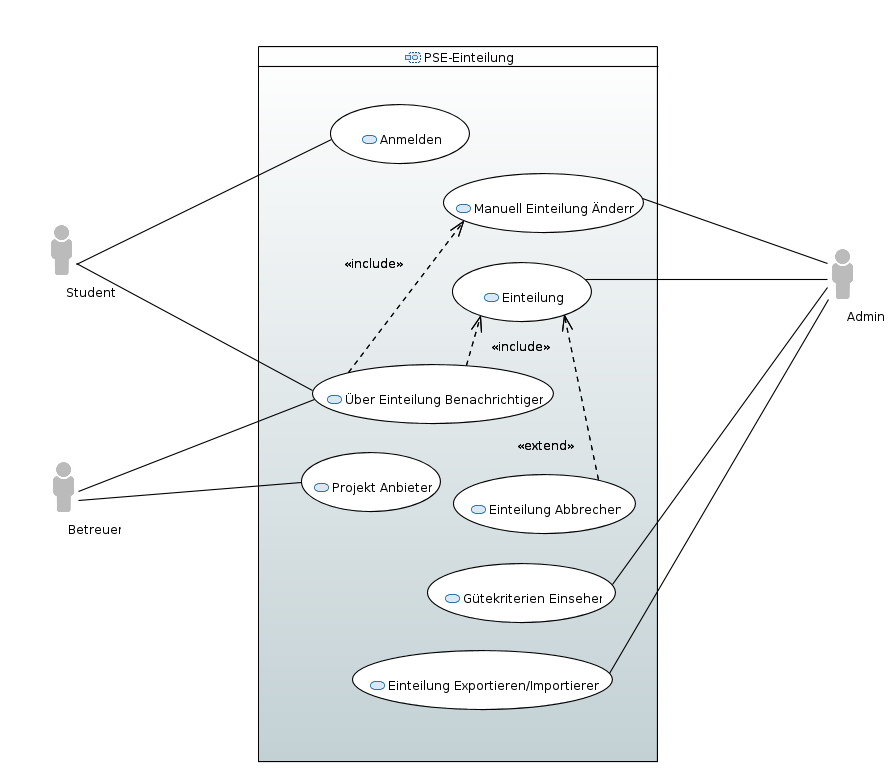
\includegraphics[width=\linewidth]{diagramme_pflichtenheft/UseCase_Diagram.PNG}
\captionof{figure}{Übersicht über die Anwendungsfälle}

\subsubsection{Studierende}

\begin{enumerate}[label=\swtLabel{S}]
	\item
    \begin{description}
  	\item[Anwendung:] Registrierung eines Studierenden
  	\item[Ziel:] Speichern der Studierendendaten in der Datenbank
  	\item[Vorbedingung:] Registrierung wurde freigeschaltet
  	\item[Nachbedingung(Erfolg):] Erfolgreiche Registrierung des Studierenden
  	\item[Nachbedingung(Fehlschlag):] Studierender ist weiterhin nicht
  	registriert
  	\item[Akteure:] Studierender
  	\item[Auslösen des Ereignisses:] Studierender will sich registrieren
  	\item[Beschreibung:]~
  	\begin{enumerate}
  	  \item[1.] Öffnen der Internetseite
      \item[2.] Klick auf Registrieren
      \item[3.] Ausfüllen der Registrierungsmaske %TODO Verweis auf Bild
      \item[4.] Abschicken der Daten
      \item[5.] Existiert der registrierte Account noch nicht, so wurde der
      Studierende der Datenbank hinzugefügt
  	\end{enumerate}
  	\item[Erweiterungen:]~
  	\begin{enumerate}
  	  \item[zu 3)] Statt der Registrierungsmaske wird hier der u-Account
  	  verwendet
  	  \item[nach 4)] Dem Studierenden wird nach dem Abschicken seiner Daten eine
  	  \\
  	  Verifikations-Email gesendet.
  	 \end{enumerate} 
  	\item[Alternativen:]~
  	\begin{enumerate}
  	  \item[5a)] Wenn doch, so wird kein weiterer Eintrag hinzugefügt, sondern
  	  die zweite Registrierung abgebrochen
  	\end{enumerate} 
  	\item[benötigte FA:] \ref{FAregistrierung}, \ref{FAstudUanmeldung},
  	\ref{FAemailverifikation}
  \end{description}
%   
  
  \item
    \begin{description}
    \item[Anwendung:] Verifikation der E-Mail
    \item[Ziel:] Verifikation der E-mail
    \item[Vorbedingung:] Studierender muss sich registriert haben und seine
    E-mail korrekt angegeben haben.
    \item[Nachbedingung(Erfolg):] Studierender kann sich nun Anmelden und hat
    Zugriff auf die Studierenden-Sicht
    \item[Nachbedingung(Fehlschlag):] Studierender kann sich nicht mit seinem
    Account anmelden
    \item[Akteure:] Studierender
    \item[Auslösen des Ereignisses:] Studierende registrieren sich und werden
    darauf hingewiesn inhre E-mail zu verifizieren.
    \item[Beschreibung:]~
    \begin{enumerate}
      \item[1.] E-mails über Drittsoftware abrufen.
      \item[2.] Klick auf den Verifikations-Link in der E-mail.      
    \end{enumerate}
    \item[Erweiterungen:] -keine-
    \item[Alternativen:] -keine-
    \item[benötigte FA:] \ref{FAemailverifikation}
      \end{description}
  
  \item
    \begin{description}
    \item[Anwendung:] Anmeldung eines Studierenden
    \item[Ziel:] Studierender wird angemeldet und kann seine Bewertungen ändern
  	\item[Vorbedingung:] Der Studierende hat sich vorher registriert
  	\item[Nachbedingung(Erfolg):] Der Studierende ist angemeldet
  	\item[Nachbedingung(Fehlschlag):] Der Studierende ist nicht angemeldet
  	\item[Akteure:] Studierender
  	\item[Auslösen des Ereignisses:] Studierender will sich anmelden
  	\item[Beschreibung:]~
  	\begin{enumerate}
  	  \item[1.] Studierender öffnet die Website
  	  \item[2.] Studierender füllt das Formular zum Anmelden aus und schickt
  	  dieses ab %TODO: Verweis auf Bild
  	  \item[3.] Sind die Anmeldedaten korrekt, so wird der Studierende zur
  	  Studierendensicht weitergeleitet
  	\end{enumerate}
  	\item[Erweiterungen:]
  	\begin{enumerate}
  	  \item[2)] Kein Formular, sondern Anmeldung über u-Account
  	\end{enumerate}    	
  	\item[Alternativen:]
	\begin{enumerate}
  	  \item[3a)] Wenn nicht, so erhält er eine Fehlermeldung
  	\end{enumerate}
  	\item[benötigte FA:] \ref{FAStudanmeldung}, \ref{FAstudUanmeldung}
  \end{description}
   
  
  \item
  \begin{description}
  \item[Anwendung:] Studierender erstellt Lerngruppe
  \item[Ziel:] Eine neue Lerngruppe ist in der Datenbank vermerkt und der Ersteller ist erstes Mitglied dieser
  	\item[Vorbedingung:] Studierender ist angemeldet und befindet sich auf der
  	Website im Studierendenportal
  	\item[Nachbedingung(Erfolg):] Die Lerngruppe wurde erfolgreich erstellt
  	\item[Nachbedingung(Fehlschlag):] Die Lerngruppe wurde nicht erstellt
  	\item[Akteure:] Studierender
  	\item[Auslösen des Ereignisses:] Wille des Studierenden
  	\item[Beschreibung:]~
  	\begin{enumerate}
  	  \item[1.] Studierender gibt Name und Passwort in das Formular zum Erstellen
  	  einer Lerngruppe ein und schickt dieses ab %TODO: Verweis einfügen
  	  \item[2.] Wenn noch keine Lerngruppe mit diesem Namen existiert, so wird
  	  die Lerngruppe in der Datenbank angelegt und der Ersteller wird erstes Mitglied
  	\end{enumerate}
  	\item[Erweiterungen:] -keine-
  	\item[Alternativen:] ~
  	\begin{enumerate}
  	  \item[2a)] Eine Lerngruppe mit diesem Namen existiert schon. Dann wird
  	  keine weitere Lerngruppe angelegt und dem Studierenden wird mitgeteilt,
  	  dass er den Namen der Lerngruppe verändern soll
  	 \end{enumerate}
  	 \item[benötigte FA:] \ref{FAcreatelerng}
  \end{description}
   
  
  \item
  \begin{description}
  \item[Anwendung:] Studierender tritt Lerngruppe bei
  \item[Ziel:] Studierender ist Mitglied einer Lerngruppe
  	\item[Vorbedingung:] Studierender ist angemeldet und befindet sich auf der
  	Website im Studierendenportal
  	\item[Nachbedingung(Erfolg):] Der Studierende ist Mitglied der Lerngruppe
  	\item[Nachbedingung(Fehlschlag):] Der Studierende ist nicht Mitglied der
  	Lerngruppe
  	\item[Akteure:] Studierender
  	\item[Auslösen des Ereignisses:] Der Studierende will einer Lerngruppe beitreten
  	\item[Beschreibung:]~
  	\begin{enumerate}
  	  \item[1.] Der Studierende gibt die Anmeldedaten der Lerngruppe in das
  	  passende Formular ein und schickt dieses ab %TODO: Verweis
  	  \item[2.] Existiert die angegebene Lerngruppe, so wird die Mitgliederliste
  	  derer um den Studierenden erweitert
  	\end{enumerate}
  	\item[Erweiterungen:]~
  	\begin{enumerate}
  	  \item[2a)] Ist die Lerngruppe schon vollständig, so wird der Studierende nicht
  	  der Gruppe zugewiesen
  	  \item[3)] Ist der Studierende nicht der Lerngruppe zugewiesen worden, so werden
  	  die zuletzt gespeicherten Bewertungen verwendet
  	  \item[4)] Der Lerngruppenersteller wird per E-Mail informiert
  	 \end{enumerate}
  	\item[Alternativen:] ~
  	\begin{enumerate}
  	  \item[2a)] Existiert keine solche Gruppe, so schlägt der Beitritt fehl und
  	  der Studierende ist kein Mitglied der Lerngruppe
  	 \end{enumerate}
  	 \item[benötigte FA:] \ref{FAjoinLerng}
  \end{description}
%   
  
  \item
  \begin{description}
  \item[Anwendung:] Studierender bewertet \glspl{Projekt}
  \item[Ziel:] Der Studierende hat eine Bewertung abgegeben
  	\item[Vorbedingung:] Der Studierende ist angemeldet und im Studierendenportal der
  	Website
  	\item[Nachbedingung(Erfolg):] Für den Studierenden ist eine Bewertung
  	eingetragen
  	\item[Nachbedingung(Fehlschlag):] Der Studierende hat keine Bewertung eingetragen
  	\item[Akteure:] Studierender
  	\item[Auslösen des Ereignisses:] Des Studierendens Wille
  	\item[Beschreibung:]~
  	 \begin{enumerate}
  	   \item[1.] Der Studierende füllt die Bewertungsmaske aus %TODO: Verweis
  	   \item[2.] Der Studierende speichert die Bewertung ab
  	 \end{enumerate}
  	\item[Erweiterungen:] -keine-
  	\item[Alternativen:] -keine-
  	\item[benötigte FA:] \ref{FAbewertung}
  \end{description}
   
  
  \item
  \begin{description}
  \item[Anwendung:] Studierender bewertet \glspl{Projekt} für eine Lerngruppe
  \item[Ziel:] Die Lerngruppe assoziiert mit dem Studierenden hat eine Bewertung
  abgegeben
  	\item[Vorbedingung:] Der Studierende ist als Leiter einer Lerngruppe angemeldet
  	und im Studierendenportal der Website
  	\item[Nachbedingung(Erfolg):] Für die Lerngruppe ist eine Bewertung eingetragen
  	\item[Nachbedingung(Fehlschlag):] Für die Lerngruppe ist keine (neue)
  	Bewertung eingetragen
  	\item[Akteure:] Studierender
  	\item[Auslösen des Ereignisses:] Des Studierendens Wille
  	\item[Beschreibung:]~
  	 \begin{enumerate}
  	   \item[1.] Der Studierende füllt die Bewertungsmaske aus
  	   \item[2.] Der Studierende schließt die Bewertung ab
  	 \end{enumerate}
  	\item[Erweiterungen:] -keine-
  	\item[Alternativen:] -keine-
  	\item[benötigte FA:] \ref{FAbewertung2}
  \end{description}
   
  
  \item
    \begin{description}
  	\item[Anwendung:] Passwort vergessen
  	\item[Ziel:] Erhalten eines neuen Passworts
  	\item[Vorbedingung:] Der Studierende hat schon einen Account
  	\item[Nachbedingung(Erfolg):] Der Studierende erhält eine E-Mail mit einem
  	neuen Passwort
  	\item[Nachbedingung(Fehlschlag):] Der Studierende erhält keine E-Mail
  	\item[Akteure:] Studierender
  	\item[Auslösen des Ereignisses:] Studierender hat sein Passwort vergessen
  	\item[Beschreibung:]~
  	\begin{enumerate}
  	  \item[1.] Öffnen der Internetseite
      \item[2.] Klick auf "Passwort vergessen"
      \item[3.] Eingabe der E-Mail Adresse
      \item[4.] Der Studierende erhält eine E-Mail mit seinem neuen Passwort
  	\end{enumerate}
  	\item[Erweiterungen:] -keine-
  	\item[Alternativen:] -keine-
  	\item[benötigte FA:] \ref{FApasswortvergessen}
  \end{description}
   
\end{enumerate}

\subsubsection{Betreuer}
\begin{enumerate} [label=\swtLabel{B}]
  \item
	 \begin{description}
		\item[Anwendung:] Betreuer meldet sich an
  		\item[Ziel:] Anmeldung des Betreuers
  		\item[Vorbedingung:] Konto des Betreuers wurde angelegt
  		\item[Nachbedingung(Erfolg):] Betreuer ist angemeldet
  		\item[Nachbedingung(Fehlschlag):] Betreuer ist nicht angemeldet
  		\item[Akteure:] Betreuer
  		\item[Auslösen des Ereignisses:] Betreuer möchte sich anmelden
  		\item[Beschreibung]~
  		\begin{enumerate}
  			\item[1.] Der Betreuer gibt seine Zugangsdaten ein
  			\item[2.] Wenn die Anmeldedaten korrekt sind, wird er auf die
  			Betreueransicht weitergeleitet
  		\end{enumerate}
  		\item[Erweiterungen:] -keine-
  		\item[Alternativen:] ~
  		\begin{enumerate}
  		  \item[2a)] Wenn nicht, erhält er eine Fehlermeldung
  		\end{enumerate}  
  		\item[benötigte FA:] \ref{FAbetreueranmeldung}
  	\end{description}
   
  
  \item
	\begin{description}
  		\item[Anwendung:] Thema erstellen/ändern
  		\item[Ziel:] Eröffnung/Änderung eines PSE-Themas
  		\item[Vorbedingung:] -keine-
  		\item[Nachbedingung(Erfolg):] Themendaten sind im System eingetragen
  		\item[Nachbedingung(Fehlschlag):] Themenfaten sind nicht im System
  		eingetragen
  		\item[Akteure:] Betreuer
  		\item[Auslösen des Ereignisses:] Betreuer möchte ein PSE-Thema ins System
  		einfügen/ändern.
  		\item[Beschreibung:]~
  	\begin{enumerate}
  	  \item[1.] Betreuer befindet sich auf der Website mit den PSE-Themen
  	  \item[2.] Existiert das Thema schon, so wählt der Betreuer dieses aus
  	  \item[3.] Betreuer füllt die Eingabemaske aus
  	  \item[4.] Betreuer speichert die neuen Daten ab
  	\end{enumerate}
  	\item[Erweiterungen:] -keine-
  	\item[Alternativen:]~
  	\begin{enumerate}
  	  \item[2a)] Wenn nicht, so fügt er ein neues hinzu
  	\end{enumerate}  
  	\item[benötigte FA:] \ref{FAbetreuer+projekt}, \ref{FAbetreuerProjektänderung}
  \end{description}

 
  \item
	\begin{description}
  		\item[Anwendung:] Gruppenbetreuer werden
  		\item[Ziel:] Betreuer einer bestimmten Gruppe werden
  		\item[Vorbedingung:] Man ist noch nicht Betreuer der ausgewählten Gruppe
  		\item[Nachbedingung(Erfolg):] Erfolgreich Betreuer der ausgewählten
  		Gruppe geworden
  		\item[Nachbedingung(Fehlschlag):] Man ist nicht Betreuer der Gruppe
  		\item[Akteure:] Betreuer
  		\item[Auslösen des Ereignisses:] Betreuer möchte sich einer Gruppe
  		zuordnen
  		\item[Beschreibung:]~
  	\begin{enumerate} 
  	  \item[1.] Betreuer befindet sich auf der Website mit den PSE-Gruppen
  	  \item[2.] Betreuer wählt die Gruppe aus, welcher er betreuen möchte
  	  \item[3.] Betreuer tritt der Gruppe bei
  	\end{enumerate}
  	\item[Erweiterungen:] -keine-
  	\item[Alternativen:] -keine-
  	\item[benötigte FA:] \ref{FAjoinBetreuer}
  \end{description}
   
  
  \item
	\begin{description}
  		\item[Anwendung:] Gruppe verlassen
  		\item[Ziel:] Eine Gruppe nicht mehr betreuen
  		\item[Vorbedingung:] Man ist Betreuer einer Gruppe, in der noch mindestens
  		ein anderer Betreuer ist.
  		\item[Nachbedingung(Erfolg):] Man betreut die Gruppe nicht länger.
  		\item[Nachbedingung(Fehlschlag):] Man ist immernoch Betreuer der Gruppe.
  		\item[Akteure:] Betreuer
  		\item[Auslösen des Ereignisses:] Betreuer möchte aus Gruppe austreten.
  		\item[Beschreibung:]~
  	\begin{enumerate} 
  	  \item[1.] Betreuer befindet sich auf der Website mit den PSE-Gruppen, die
  	  er betreut.
  	  \item[2.] Betreuer wählt die Gruppe aus, welche er verlassen möchte.
  	  \item[3.] Betreuer verlässt die Gruppe.
  	\end{enumerate}
  	\item[Erweiterungen:] -keine-
  	\item[Alternativen:] -keine-
  	\item[benötigte FA:] \ref{FAleaveBetreuer}
  \end{description}
   
  
  \item
    \begin{description}
  	\item[Anwendung:] Noten für Gruppenteilnehmer eintragen
  	\item[Ziel:] Speichern der Noten in der Datenbank
  	\item[Vorbedingung:] Gruppe hat Studierenden als Teilnehmer
  	\item[Nachbedingung(Erfolg):] Eintragung/Änderung der Noten
  	\item[Nachbedingung(Fehlschlag):] Notenänderung wird verworfen
  	\item[Akteure:] Betreuer
  	\item[Auslösen des Ereignisses:] Betreuer möchte Noten eintragen
  	\item[Beschreibung:]~
  	\begin{enumerate} 
  	  \item[1.] Betreuer befindet sich auf der Website mit der Notenübersicht
  	  \item[2.] Betreuer trägt neue Noten für eine beliebige Phase ein oder
  	  ändert bestehende Noten.
  	\end{enumerate}
  	\item[Erweiterungen:] -keine-
  	\item[Alternativen] -keine-
  	\item[benötigte FA:] \ref{FAbetreuernoten}
  \end{description}
   
\end{enumerate}


\subsubsection{Administrator}
\begin{enumerate} [label=\swtLabel{A}]
  \item
    \begin{description}
  	\item[Anwendung:] Hinzufügen/Ändern eines Projekts
  	\item[Ziel:] Einfügen/Änderung von Projektdaten in der Datenbank
  	\item[Vorbedingung:] -keine-
  	\item[Nachbedingung(Erfolg):] Neue Projektdaten sind eingetragen
  	\item[Nachbedingung(Fehlschlag):] Neue Projektdaten sind nicht eingetragen
  	\item[Akteure:] Administrator, Institut
  	\item[Auslösen des Ereignisses:] Administrator bekommt Projektdaten von einem
  	Institut\\ vorgelegt
  	\item[Beschreibung:]~
  	\begin{enumerate} 
  	  \item[1.] Projektübersicht öffnen
  	  \item[2.] Wenn das Projekt schon existiert, so werden die Projektdaten
  	  verglichen
  	  \item[3.] Stimmen die Projektdaten nicht überein, so werden die betroffenen
  	  Daten\\ angepasst
  	  \item[4.] Durch Abspeichern der Eingaben werden die Daten in der Datenbank
  	  angepasst
  	\end{enumerate}
  	\item[Erweiterungen:] -keine-
  	\item[Alternativen:]~
  	\begin{enumerate}
  	  \item[2a)] Wenn nicht, dann wird das Projekt neu angelegt
  	  \item[3a)] Falls doch, so ist dieser Anwendungsfall abgeschlossen
  	\end{enumerate} 
  	\item[benötigte FA:] \ref{FAadmin+projekt}, \ref{FAadminProjektänderung}
  \end{description}
   
  
  \item
  \begin{description}
  \item[Anwendung:] Löschen eines Projekts
  \item[Ziel:] Löschen eines Projekts in der Datenbank
  	\item[Vorbedingung:] Projekt existiert bereits in der Datenbank und die
  	Studierenden konnten noch keine Bewertungen abgeben
  	\item[Nachbedingung(Erfolg):] Projekt ist aus der Datenbank entfernt
  	\item[Nachbedingung(Fehlschlag):] Projekt ist immernoch in der Datenbank
  	\item[Akteure:] Administrator, Institut
  	\item[Auslösen des Ereignisses:] Institut zieht ein Projekt zurück oder es
  	fehlen Daten bei Beginn der Einteilung
  	\item[Beschreibung:]~
  	\begin{enumerate} 
  	  \item[1.] Projektübersicht öffnen
  	  \item[2.] Projekt aus Liste entfernen
  	  \item[3.] Projektdaten werden aus der Datenbank entfernt
  	\end{enumerate}
  	\item[Erweiterungen:] -keine-
  	\item[Alternativen:] -keine-
  	\item[benötigte FA:] \ref{FAadmin-Projekt}
  \end{description}
   
  
  \item
  \begin{description}
  \item[Anwendung:] Teameinteilung
  \item[Ziel:] Finden einer Teameinteilung nach ausgewählten Parametern
  	\item[Vorbedingung:] Alle \glspl{Projekt} in der Datenbank sind vollständig
  	\item[Nachbedingung(Erfolg):] Es wurde eine Teameinteilung gefunden
  	\item[Nachbedingung(Fehlschlag):] Es wurde keine Teameinteilung gefunden
  	\item[Akteure:] Administrator
  	\item[Auslösen des Ereignisses:] Entscheidung des Administrators bzw.
  	zeitliche Deadline
  	\item[Beschreibung:]~
  	\begin{enumerate} 
  	  \item[1.] Einstellen der Parameter nach den eingeteilt werden soll
  	  \item[2.] Starten der Berechnung über Schaltfläche
  	  \item[3.] Sind alle \glspl{Projekt} vollständig angegeben, so startet die
  	  Berechnung
  	  \item[4.] Nach Abschluss der Berechnung wird das Ergebnis inklusive
  	  eingestellter Parameter abgespeichert.
  	\end{enumerate}
  	\item[Erweiterungen:] -keine-
  	\item[Alternativen:] ~
  	\begin{enumerate}
  	  \item[3a)] Wenn nicht, so startet die Berechnung nicht und der Fall ist
  	  beendet
  	  \item[4a)] Hier ist auch ein frühzeitiger Abbruch durch den Administrator
  	  möglich. Dies wird im Ergebnis vermerkt.
  	 \end{enumerate}  
  	 \item[benötigte FA:] \ref{FAadminparameter},
  	 \ref{FAadminEinteilungstart}, \ref{FAabbruch}
  \end{description}
   
  
  \item
  \begin{description}
  \item[Anwendung:] Finale Auswahl der Einteilung
  \item[Ziel:] Finden der bestmöglichen Teameinteilung
  	\item[Vorbedingung:] Es wurde mindestens eine Berechnung durchgeführt
  	\item[Nachbedingung(Erfolg):] Es wurde eine Teameinteilung ausgewählt
  	\item[Nachbedingung(Fehlschlag):] Es wurde keine Teameinteilung ausgewählt
  	\item[Akteure:] Administrator
  	\item[Auslösen des Ereignisses:] Entscheidung des Administrators bzw.
  	zeitliche Deadline
  	\item[Beschreibung:]~
  	\begin{enumerate} 
  	  \item[1.] Der Administrator wählt eine der berechneten Einteilung final aus
  	  \item[2.] Wurde ein Studierender zugewiesen, so wird seinem
  	  Datenbankeintrag sein Team hinzugefügt
  	\end{enumerate}
  	\item[Erweiterungen:]~
  	\begin{enumerate}
  	  \item[nach 2)] Betreuer werden über ihre Teams informiert
  	  \item[nach 2)] Die Studierenden werden über ihre Einteilung informiert
  	 \end{enumerate}
  	\item[Alternativen:] ~
  	\begin{enumerate}
  	  \item[2a)] Wird ein Studierender nicht zugewiesen, so wird dies ebenfalls
  	  in der Datenbank vermerkt
  	 \end{enumerate}  
  	 \item[benötigte FA:] \ref{FAadminÜbersicht}, \ref{FAadminAuswahl},
  	 \ref{FAadminBenachrichtigen}
  \end{description}
   
  
  \item
  \begin{description}
  \item[Anwendung:] Einteilung eines Studierenden
  \item[Ziel:] Manuelle Einteilung eines Studierenden
  	\item[Vorbedingung:] Automatische Teameinteilung ist abgeschlossen
  	\item[Nachbedingung(Erfolg):] Der Studierende wurde hinzugefügt
  	\item[Nachbedingung(Fehlschlag):] Der Studierende wurde nicht hinzugefügt
  	\item[Akteure:] Administrator, Studierender
  	\item[Auslösen des Ereignisses:] Studierender meldet sich beim Administrator
  	\item[Beschreibung:]~
  	 \begin{enumerate} 
  	   \item[1.] Wenn sich der Studierende noch nicht im System befindet
  	   überprüft der Administrator, ob die Anforderungen für das PSE erfüllt sind
  	   \item[2.] Hat der Studierende die Anforderungen erfüllt, so versucht der
  	   Administrator ihn einem Team zuzuteilen
  	   \item[3.] Hat der Administrator ein Team gefunden so fügt er den
  	   Studierenden über eine Eingabemaske dem System hinzu
  	 \end{enumerate}
  	\item[Erweiterungen:]~
  	 \begin{enumerate}
  	   \item [nach 3)] Betreuer, sowie andere Mitglieder des Projekts, werden
  	   über das neue Mitglied per E-Mail informiert 
  	 \end{enumerate}  
  	\item[Alternativen:] ~
  	 \begin{enumerate}
  	  \item[1a)] Falls doch, so wurde er schon vorher abgelehnt/nicht zugewiesen
  	  und wird nicht eingeteilt. Dieser Fall ist damit abgeschlossen
  	  \item [2a)] Falls er die Anforderungen nicht erfüllt, so wird er auch nicht
  	  zugeteilt und dieser Fall ist abgeschlossen
  	 \end{enumerate}  
  	 \item[benötigte FA:] \ref{FAadmin+Stud}
  \end{description}
   
  
  \item
  \begin{description}
  \item[Anwendung:] Erstellen eines Betreueraccounts
  \item[Ziel:] Hinzufügen eines Betreuers in das System
  	\item[Vorbedingung:] -keine-
  	\item[Nachbedingung(Erfolg):] Der Betreueraccount wurde erstellt
  	\item[Nachbedingung(Fehlschlag):] Der Betreueraccount wurde nicht erstellt
  	\item[Akteure:] Administrator
  	\item[Auslösen des Ereignisses:] Betreuer benötigt Account
  	\item[Beschreibung:]~
  	 \begin{enumerate} 
  	   \item[1.] Der Administrator öffnet die Maske zum Erstellen eines
  	   Betreueraccounts  
  	   \item[2.] Der Administrator füllt die Maske aus und schickt sie ausgefüllt
  	   ab
  	   \item[3.] Wenn noch kein Account mit dem angegebenen Namen existiert, so
  	   wird der neue Account der Datenbank hinzugefügt
  	 \end{enumerate} 
  	\item[Erweiterungen:]~
  	 \begin{enumerate}
  	   \item[4)] Der Betreuer erhält seine Zugangsdaten per E-Mail
  	 \end{enumerate}  
  	\item[Alternativen:] ~
  	 \begin{enumerate}
  	  \item[3a)] Falls doch, so wird eine Fehlermeldung angezeigt
  	 \end{enumerate}  
  	 \item[benötigte FA:] \ref{FAadminCreateAccounts}
  \end{description}
  
\end{enumerate}  
\subsection{Objektmodelle}

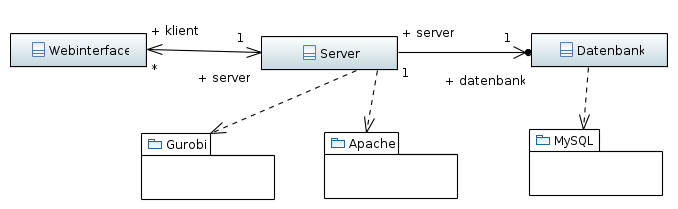
\includegraphics[width=\linewidth]{diagramme_pflichtenheft/ClassDiagram.PNG}
\captionof{figure}{Schematischer Aufbau des Produkts}

%TODO Brauchen wir das? \subsection{Dynamische Modelle}

\subsection{Benutzerschnittstelle}
\begin{enumerate}
  \item Es ist eine Benutzung rein über ein Web-Interface vorgesehen
  \item Es sind drei Sichten zu unterscheiden:
        \begin{itemize}
          \item die Sicht des Studierenden
          \item die Sicht des Betreuers
          \item die Sicht des Administrators
        \end{itemize}
  \item Die jeweiligen sichten sind erst nach der Anmeldung einzusehen 
  \item Studierende dürfen nur auf ihre eigenen Daten und falls sie in einer
  Lerngruppe sind auf die Daten dieser zugreifen
\subsubsection{GUI}
{\centering
\fbox{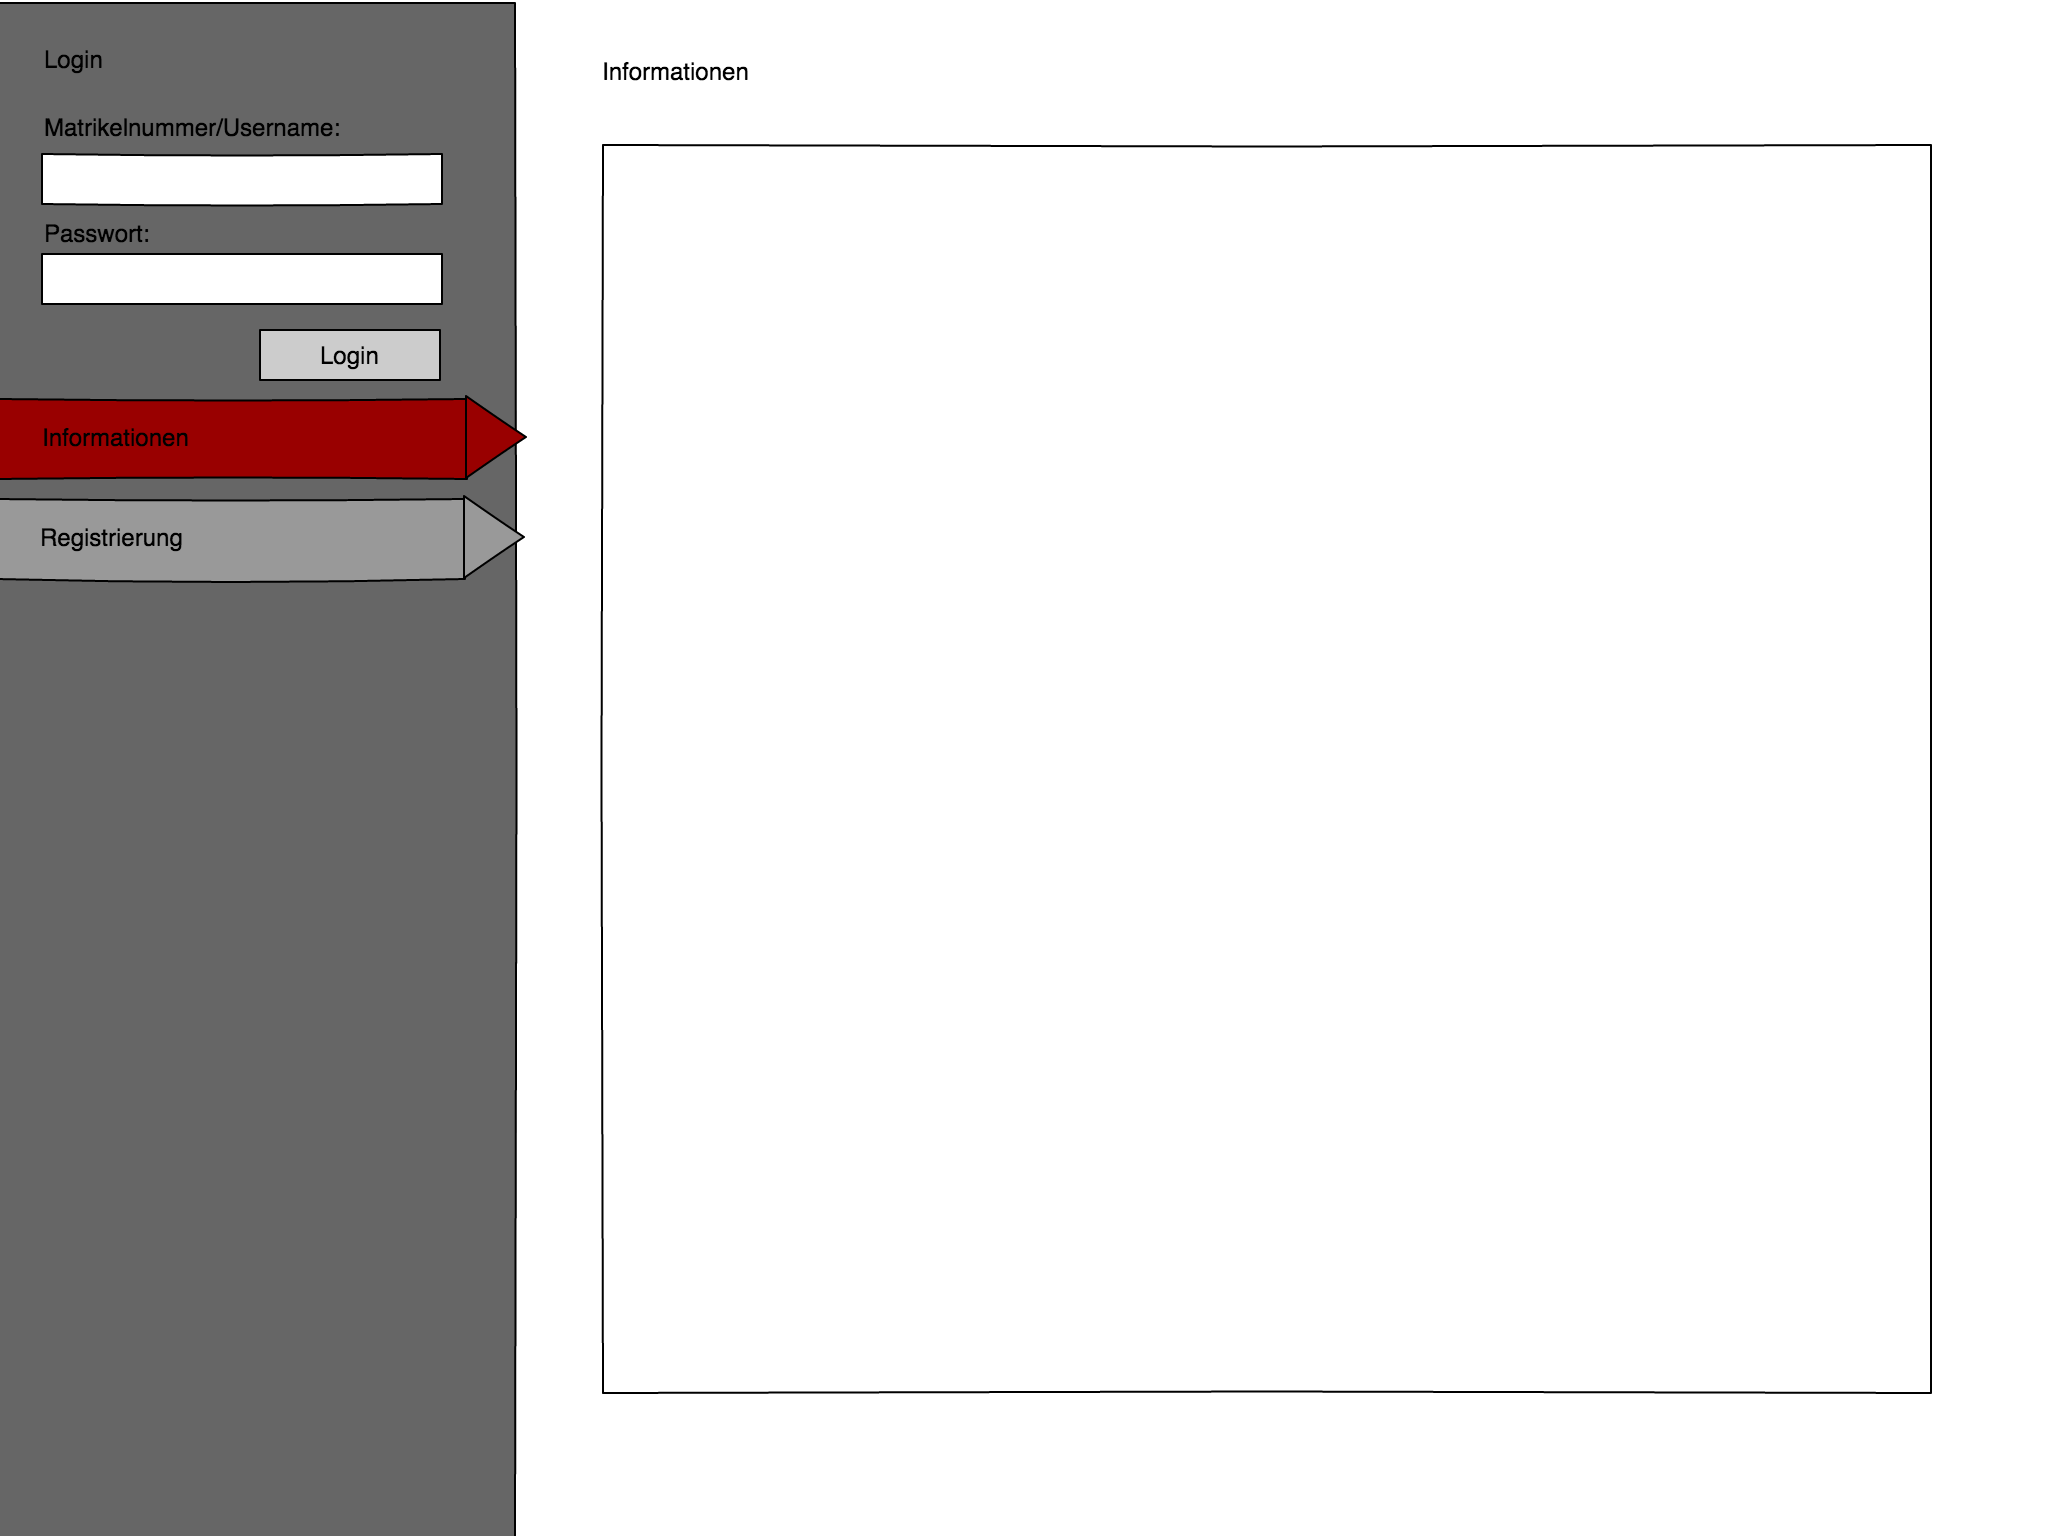
\includegraphics[width=\textwidth,
keepaspectratio=true]{gui/index.png}}
\captionof{figure}{Startseite}


\setlength{\textheight}{297mm}
\setlength{\headheight}{3mm}
\fbox{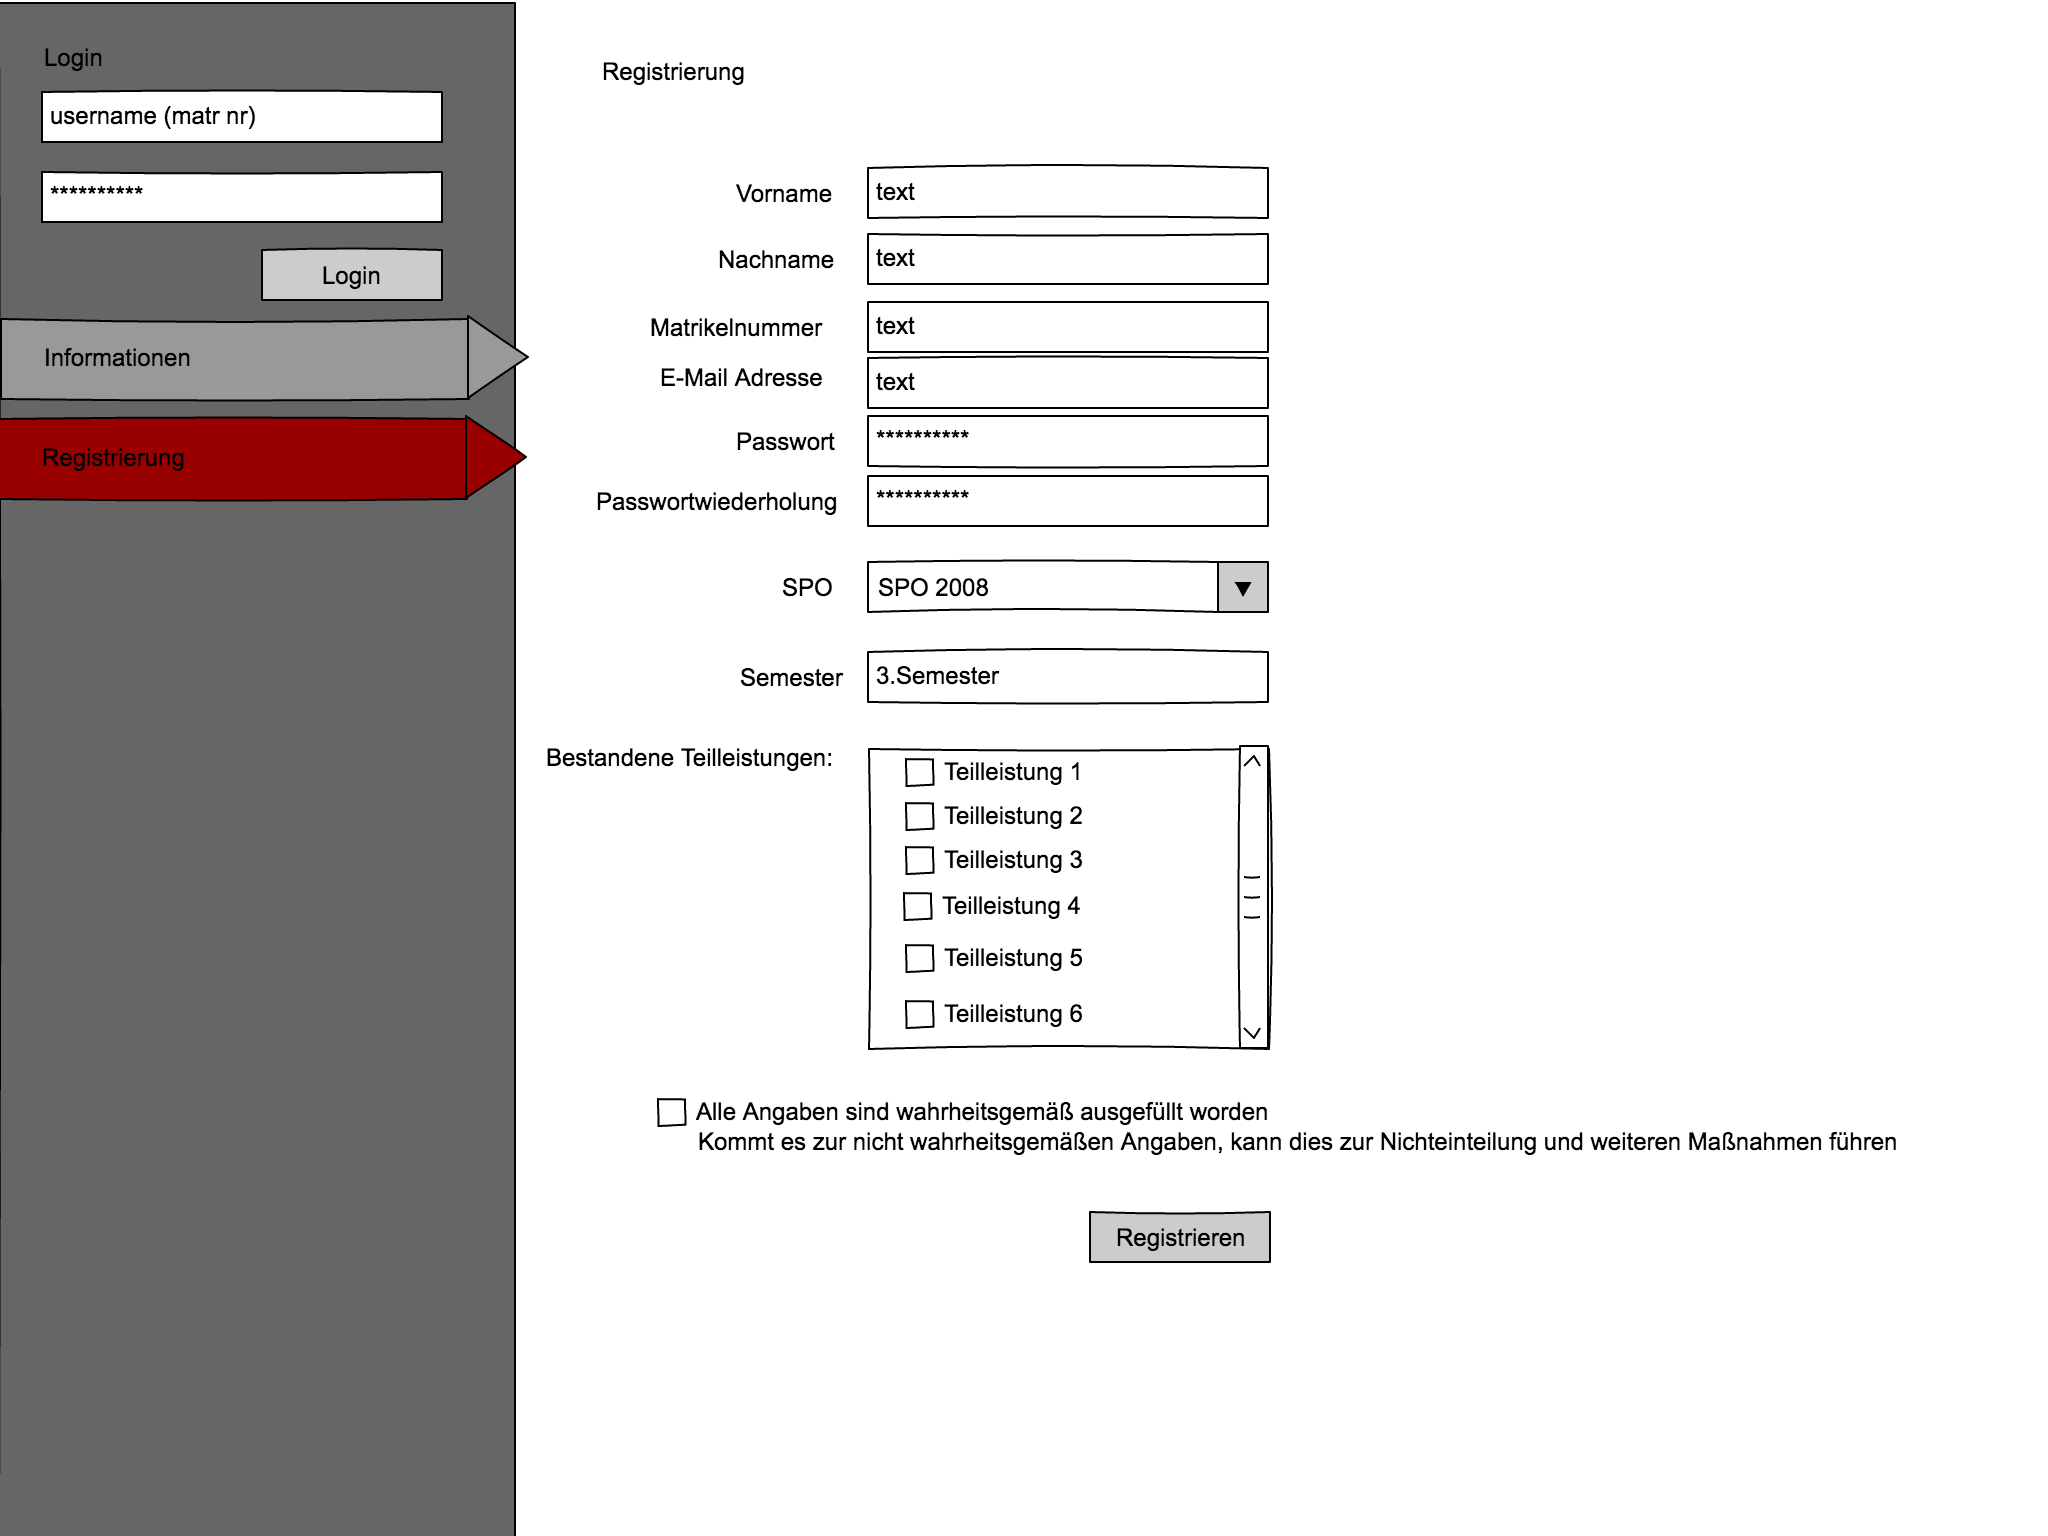
\includegraphics[width=\textwidth,
keepaspectratio=true]{gui/registrierung.png}}
\captionof{figure}{Registrierungsansicht}
\thispagestyle{empty}

\fbox{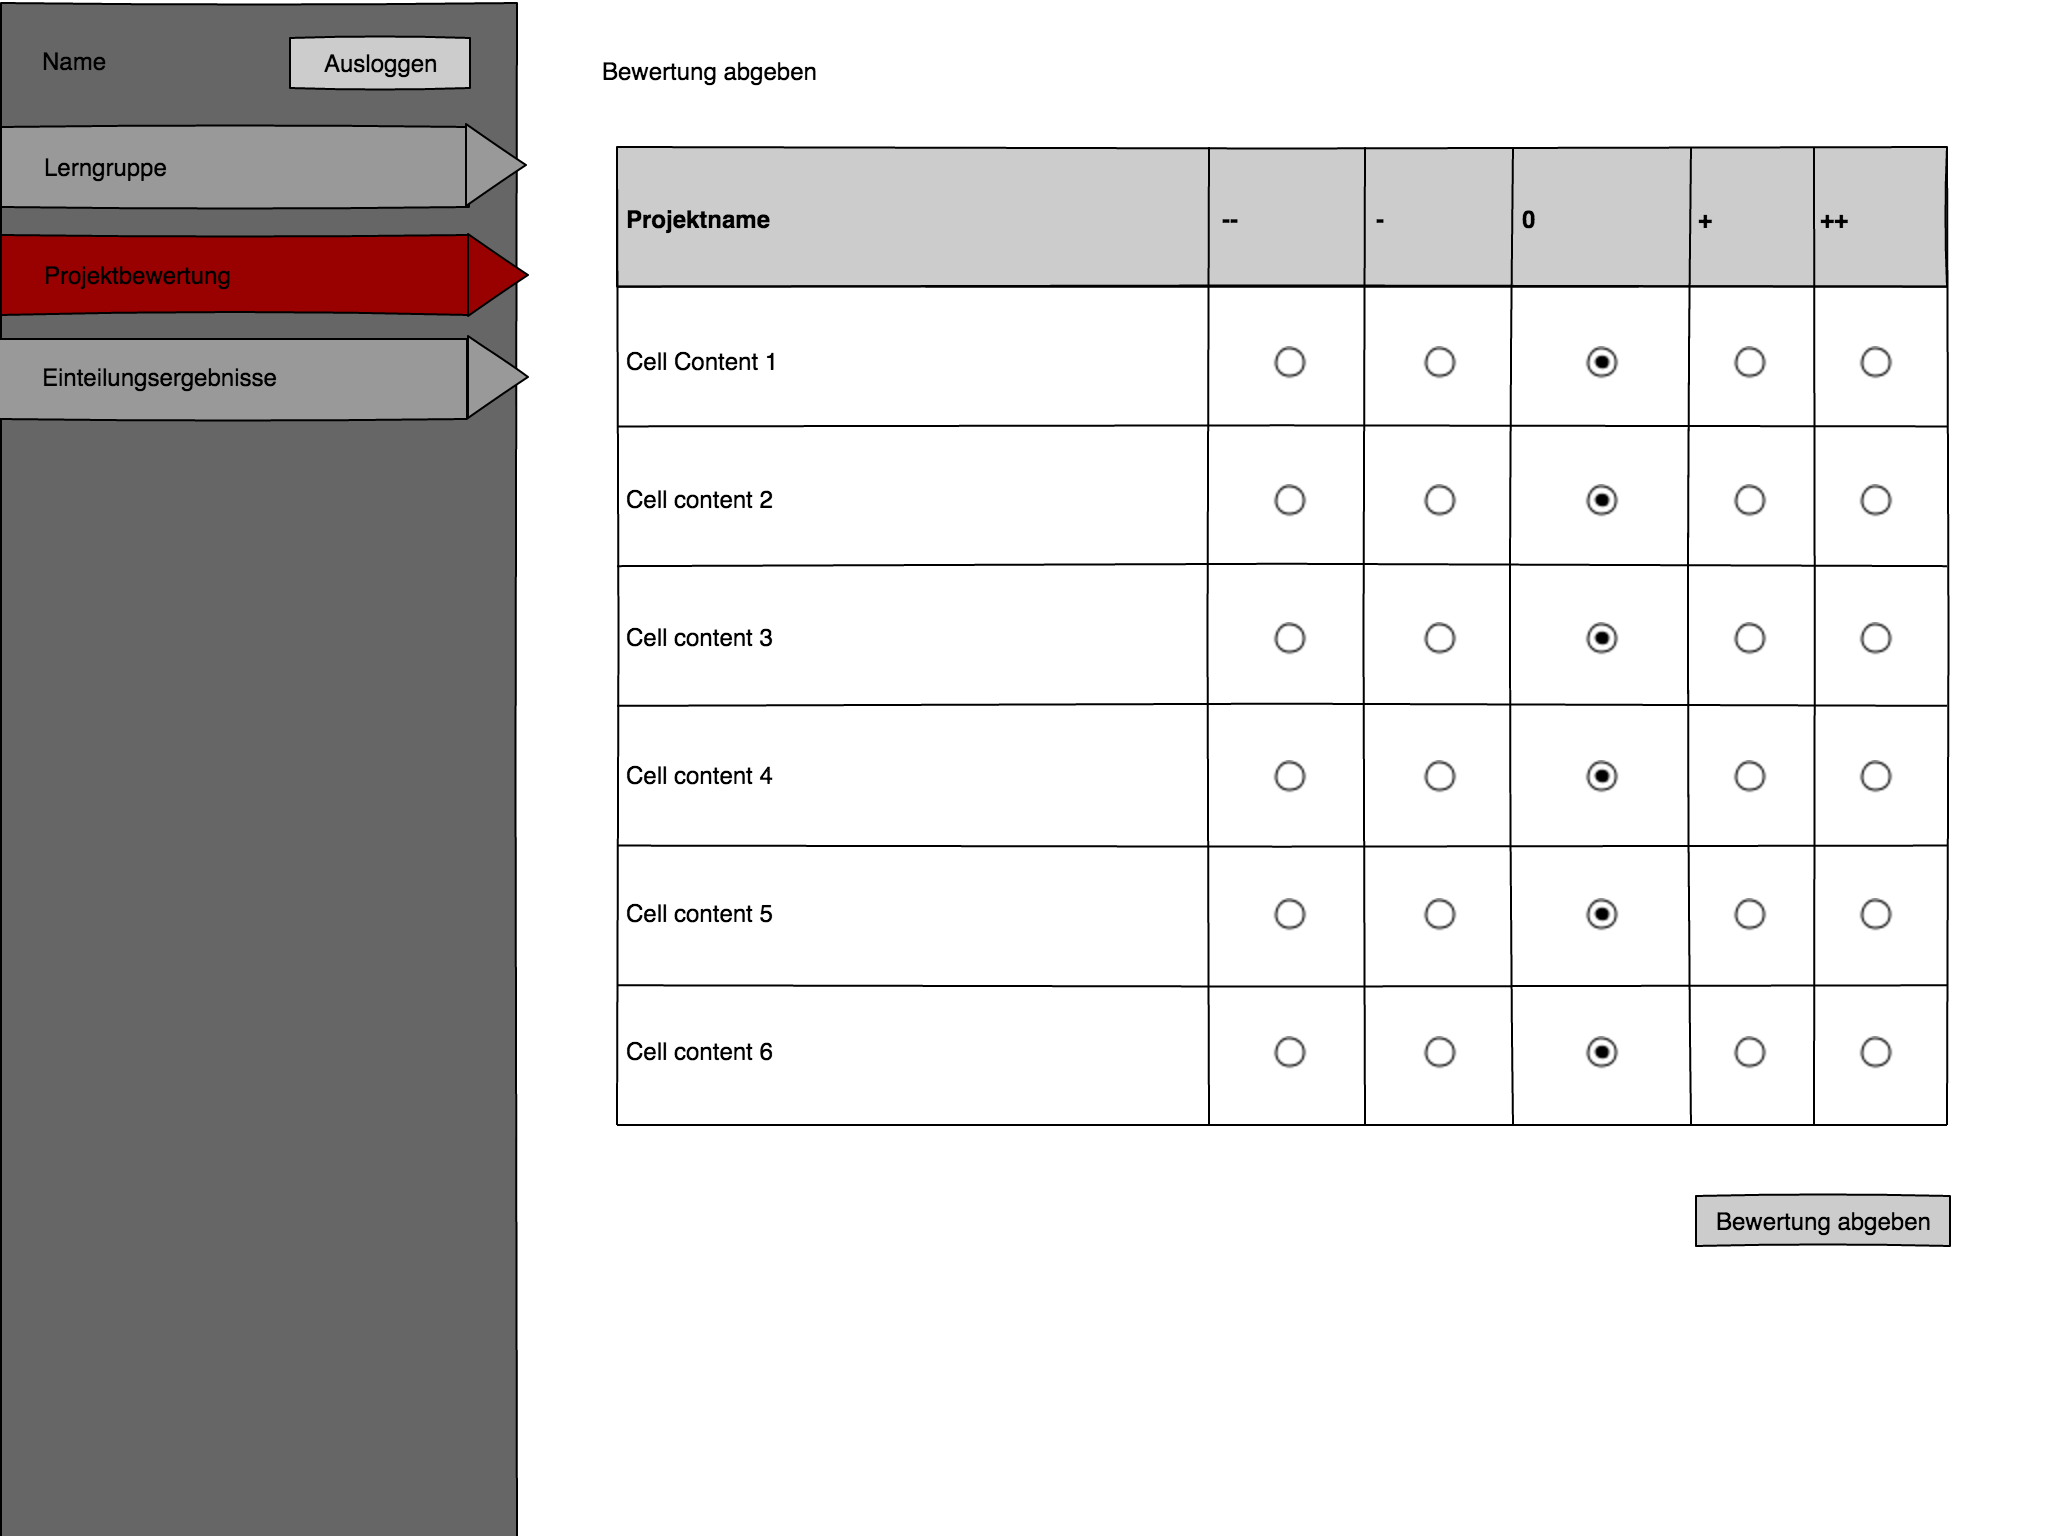
\includegraphics[width=\textwidth,
keepaspectratio=true]{gui/studentbewertung.png}}
\captionof{figure}{Bewertungsmaske}

\fbox{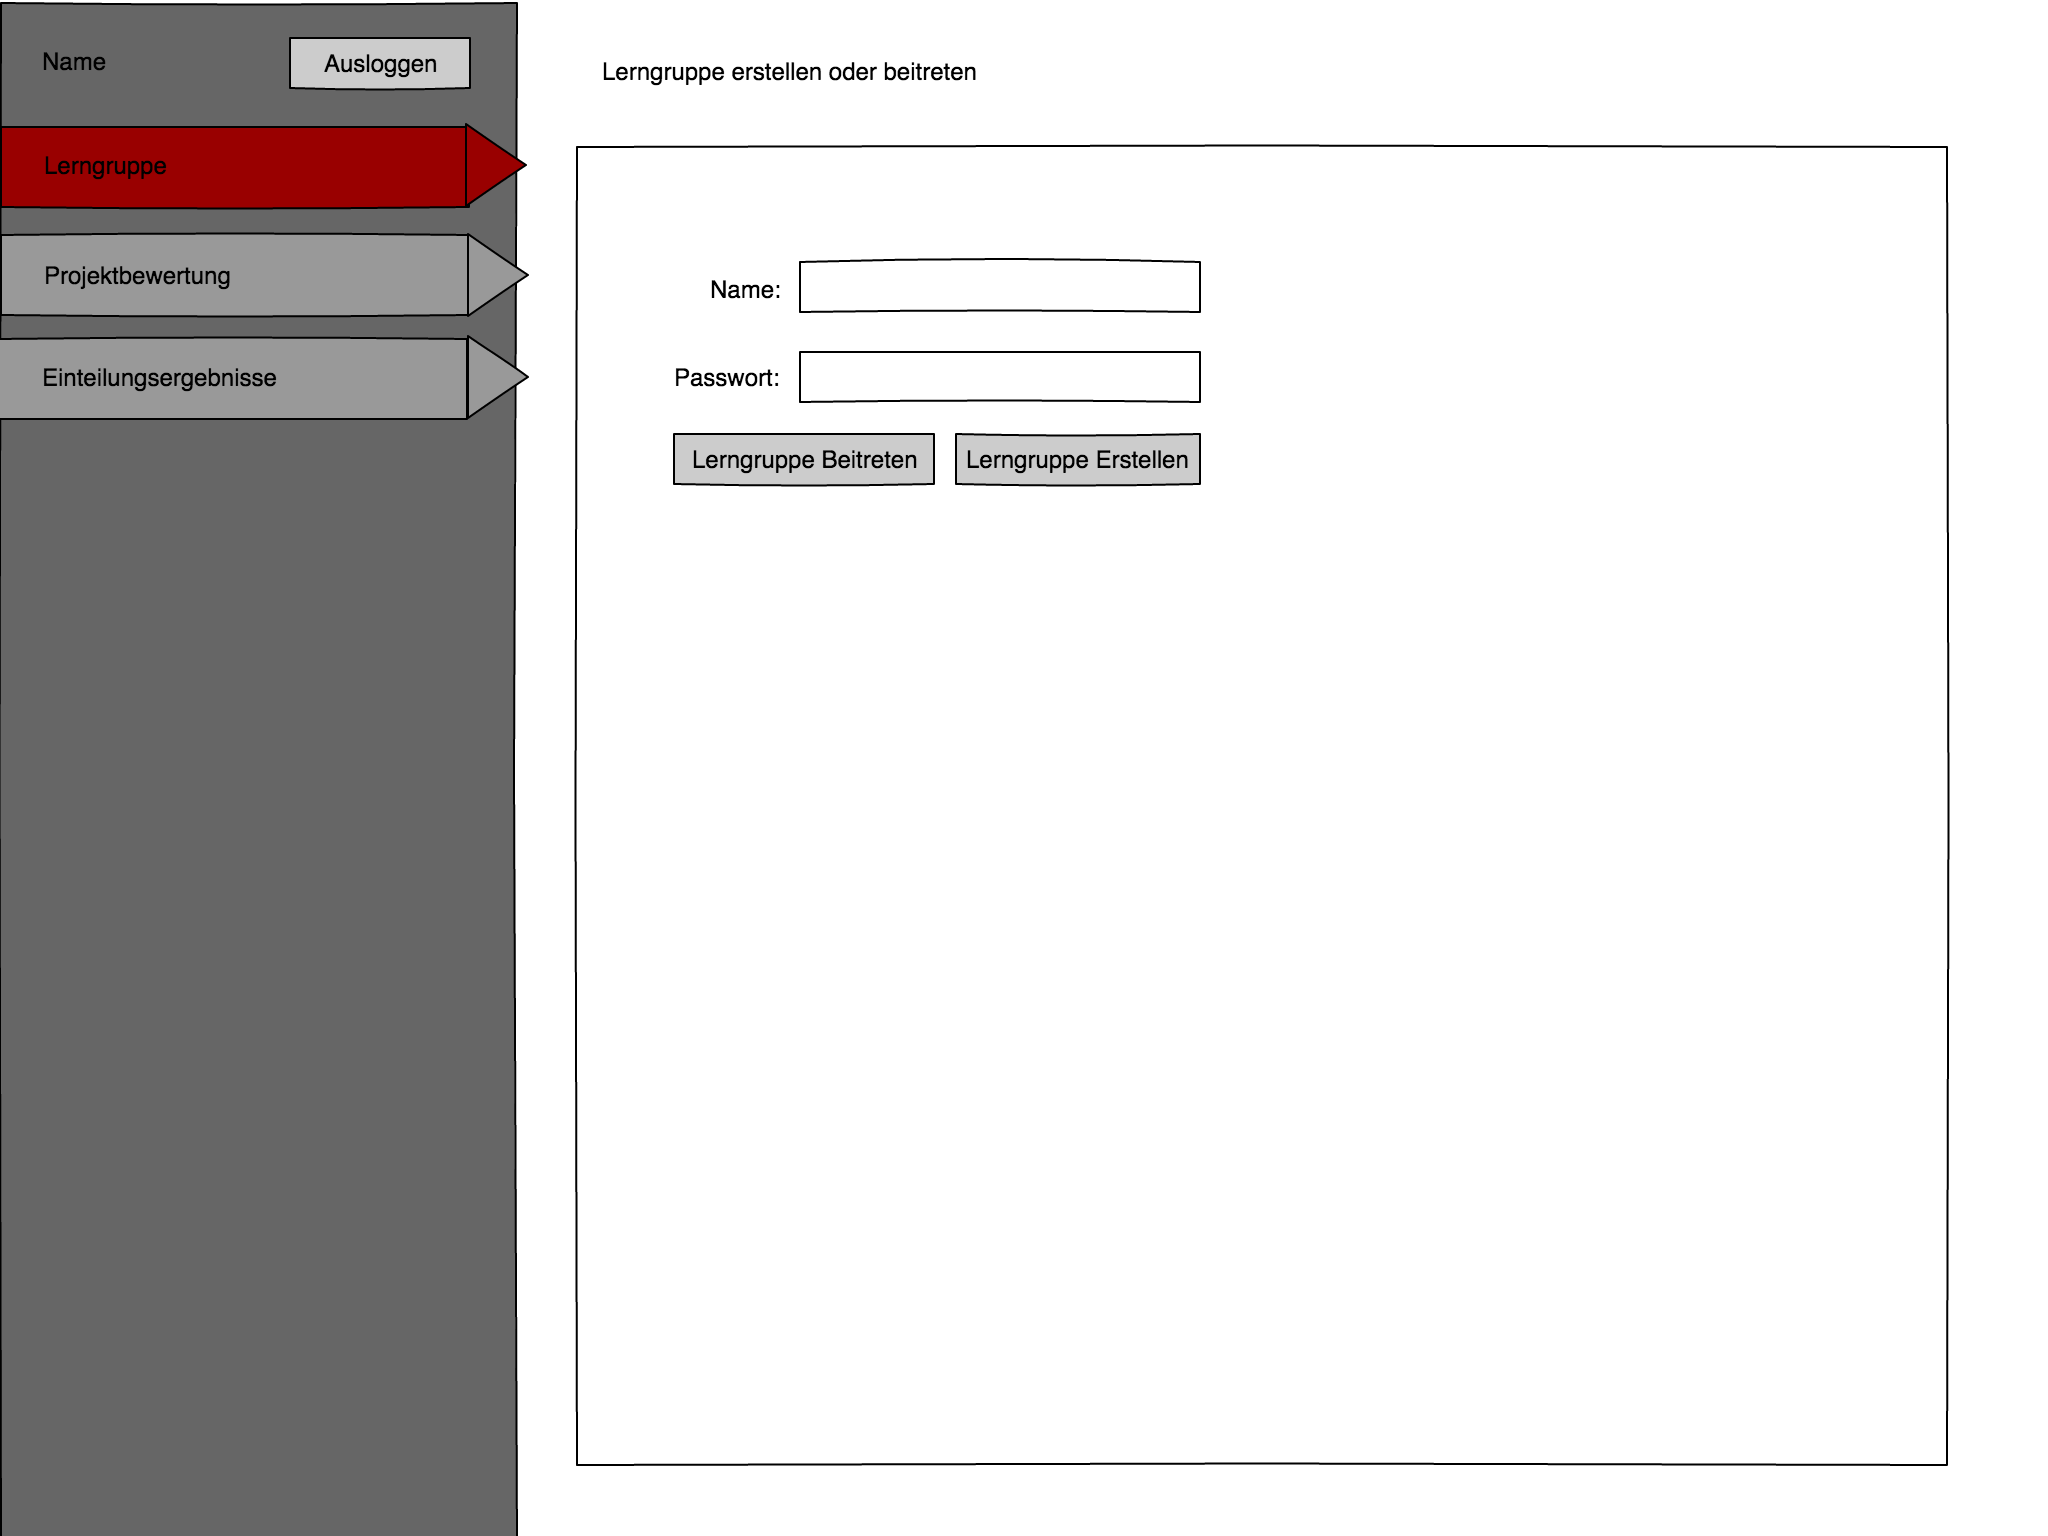
\includegraphics[width=\textwidth,
keepaspectratio=true]{gui/studentlerngruppe.png}}
\captionof{figure}{Anmeldung zu Lerngruppe}
\medskip
\fbox{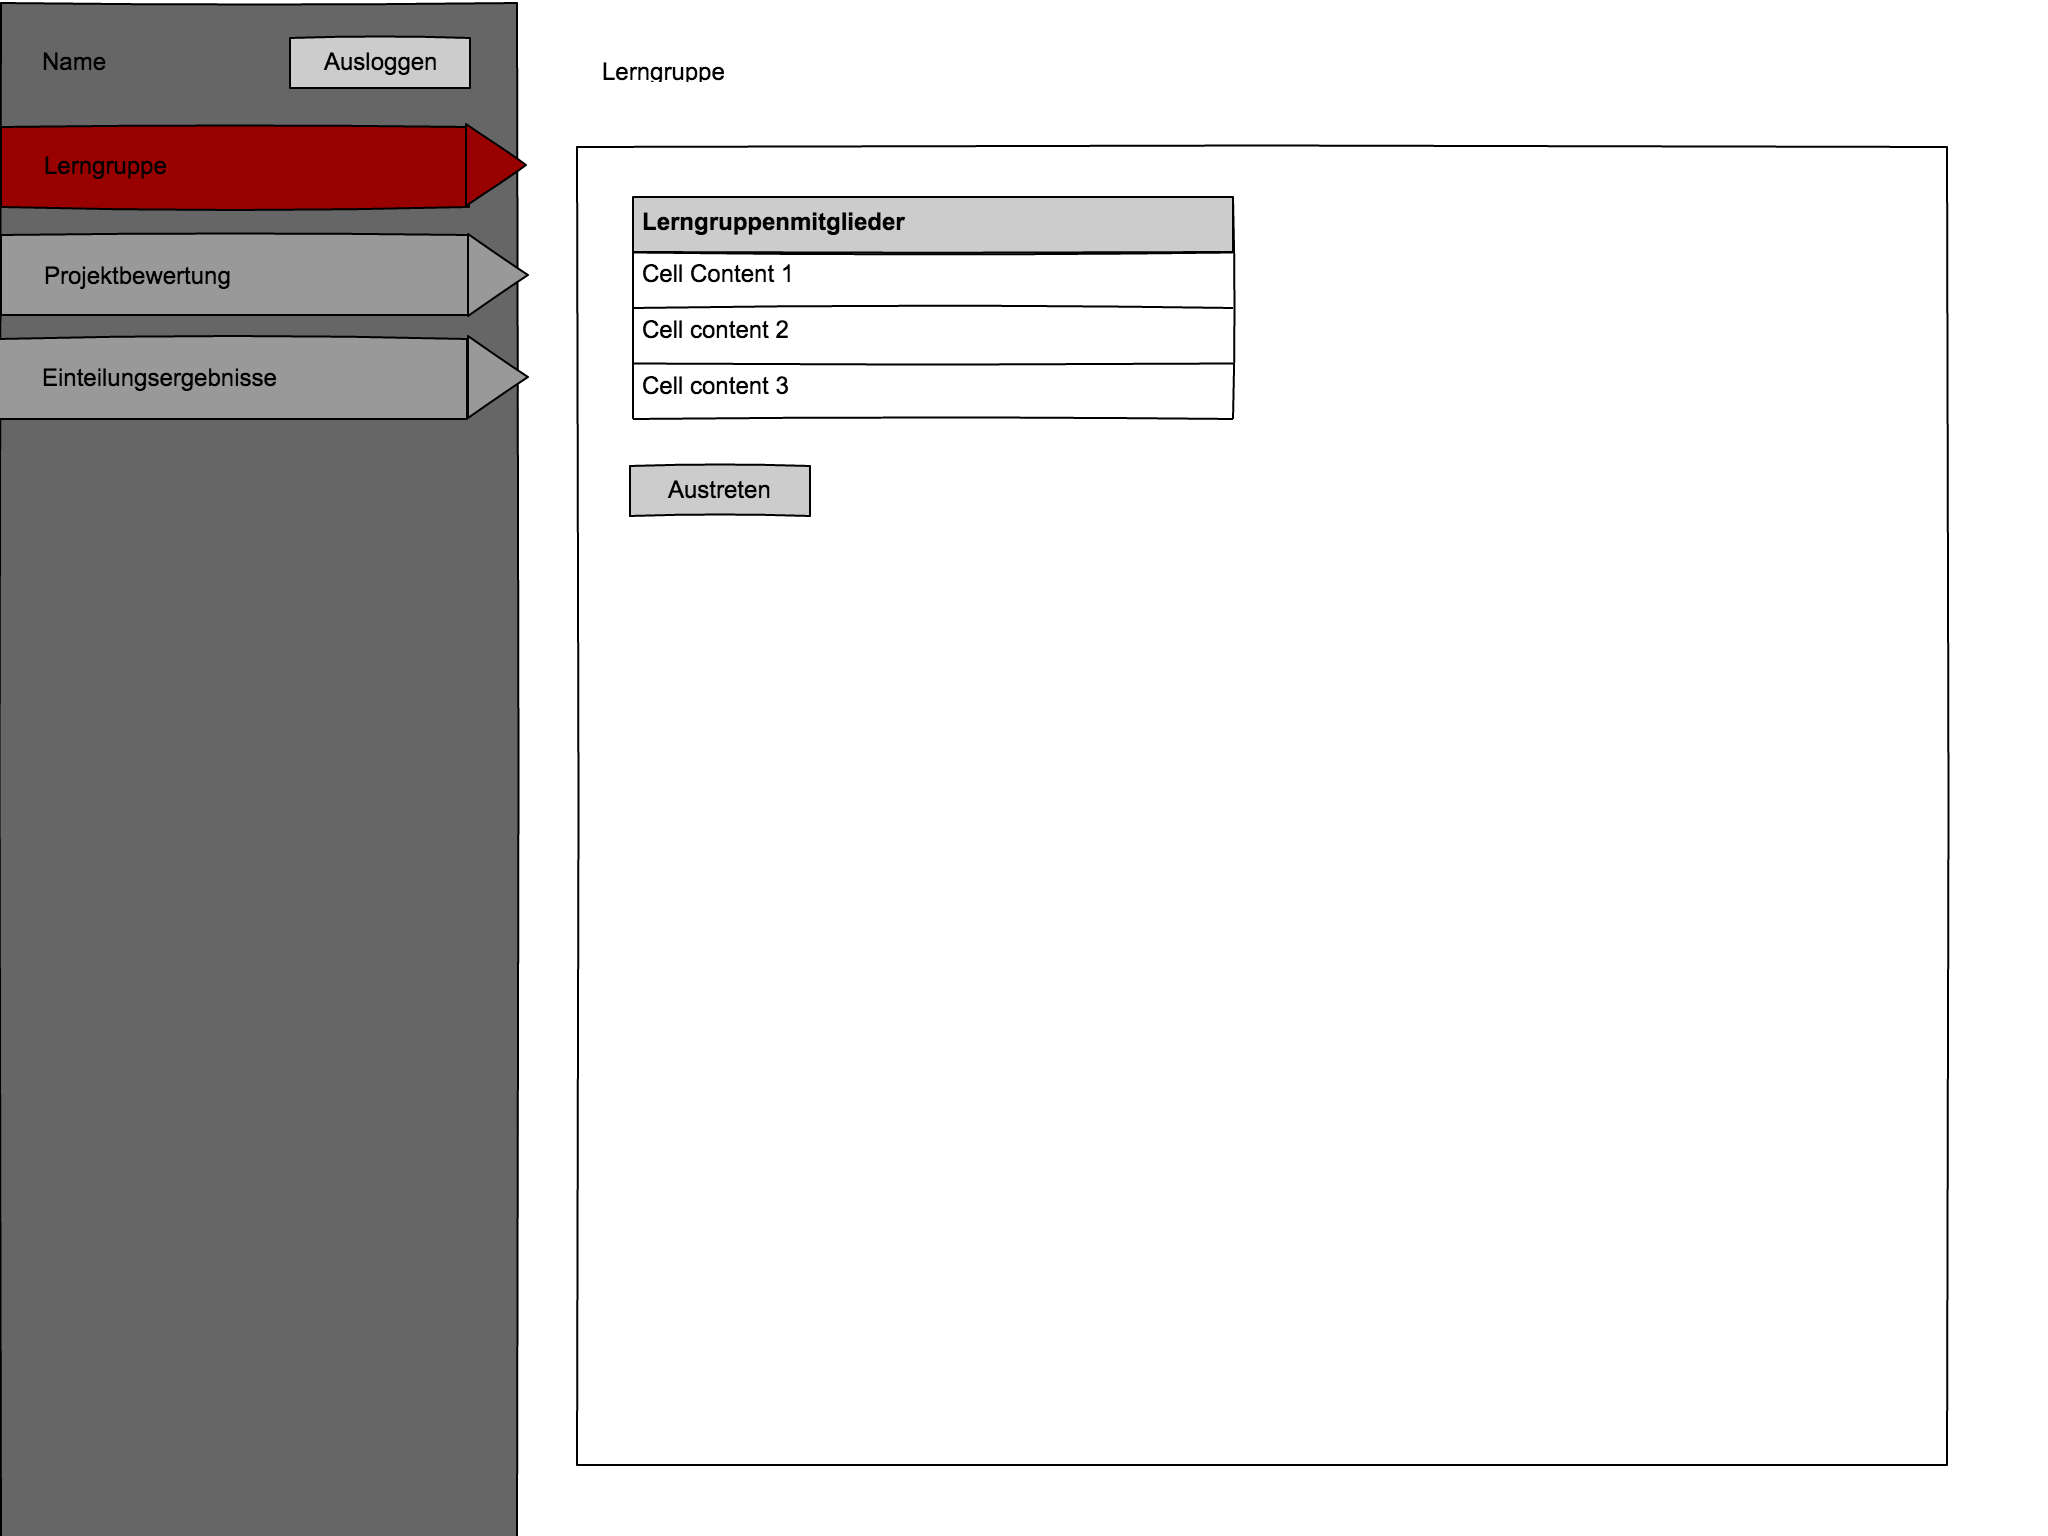
\includegraphics[width=\textwidth,
keepaspectratio=true]{gui/studentlerngruppeingr.png}}
\captionof{figure}{Lerngruppenübersicht}
\medskip
\fbox{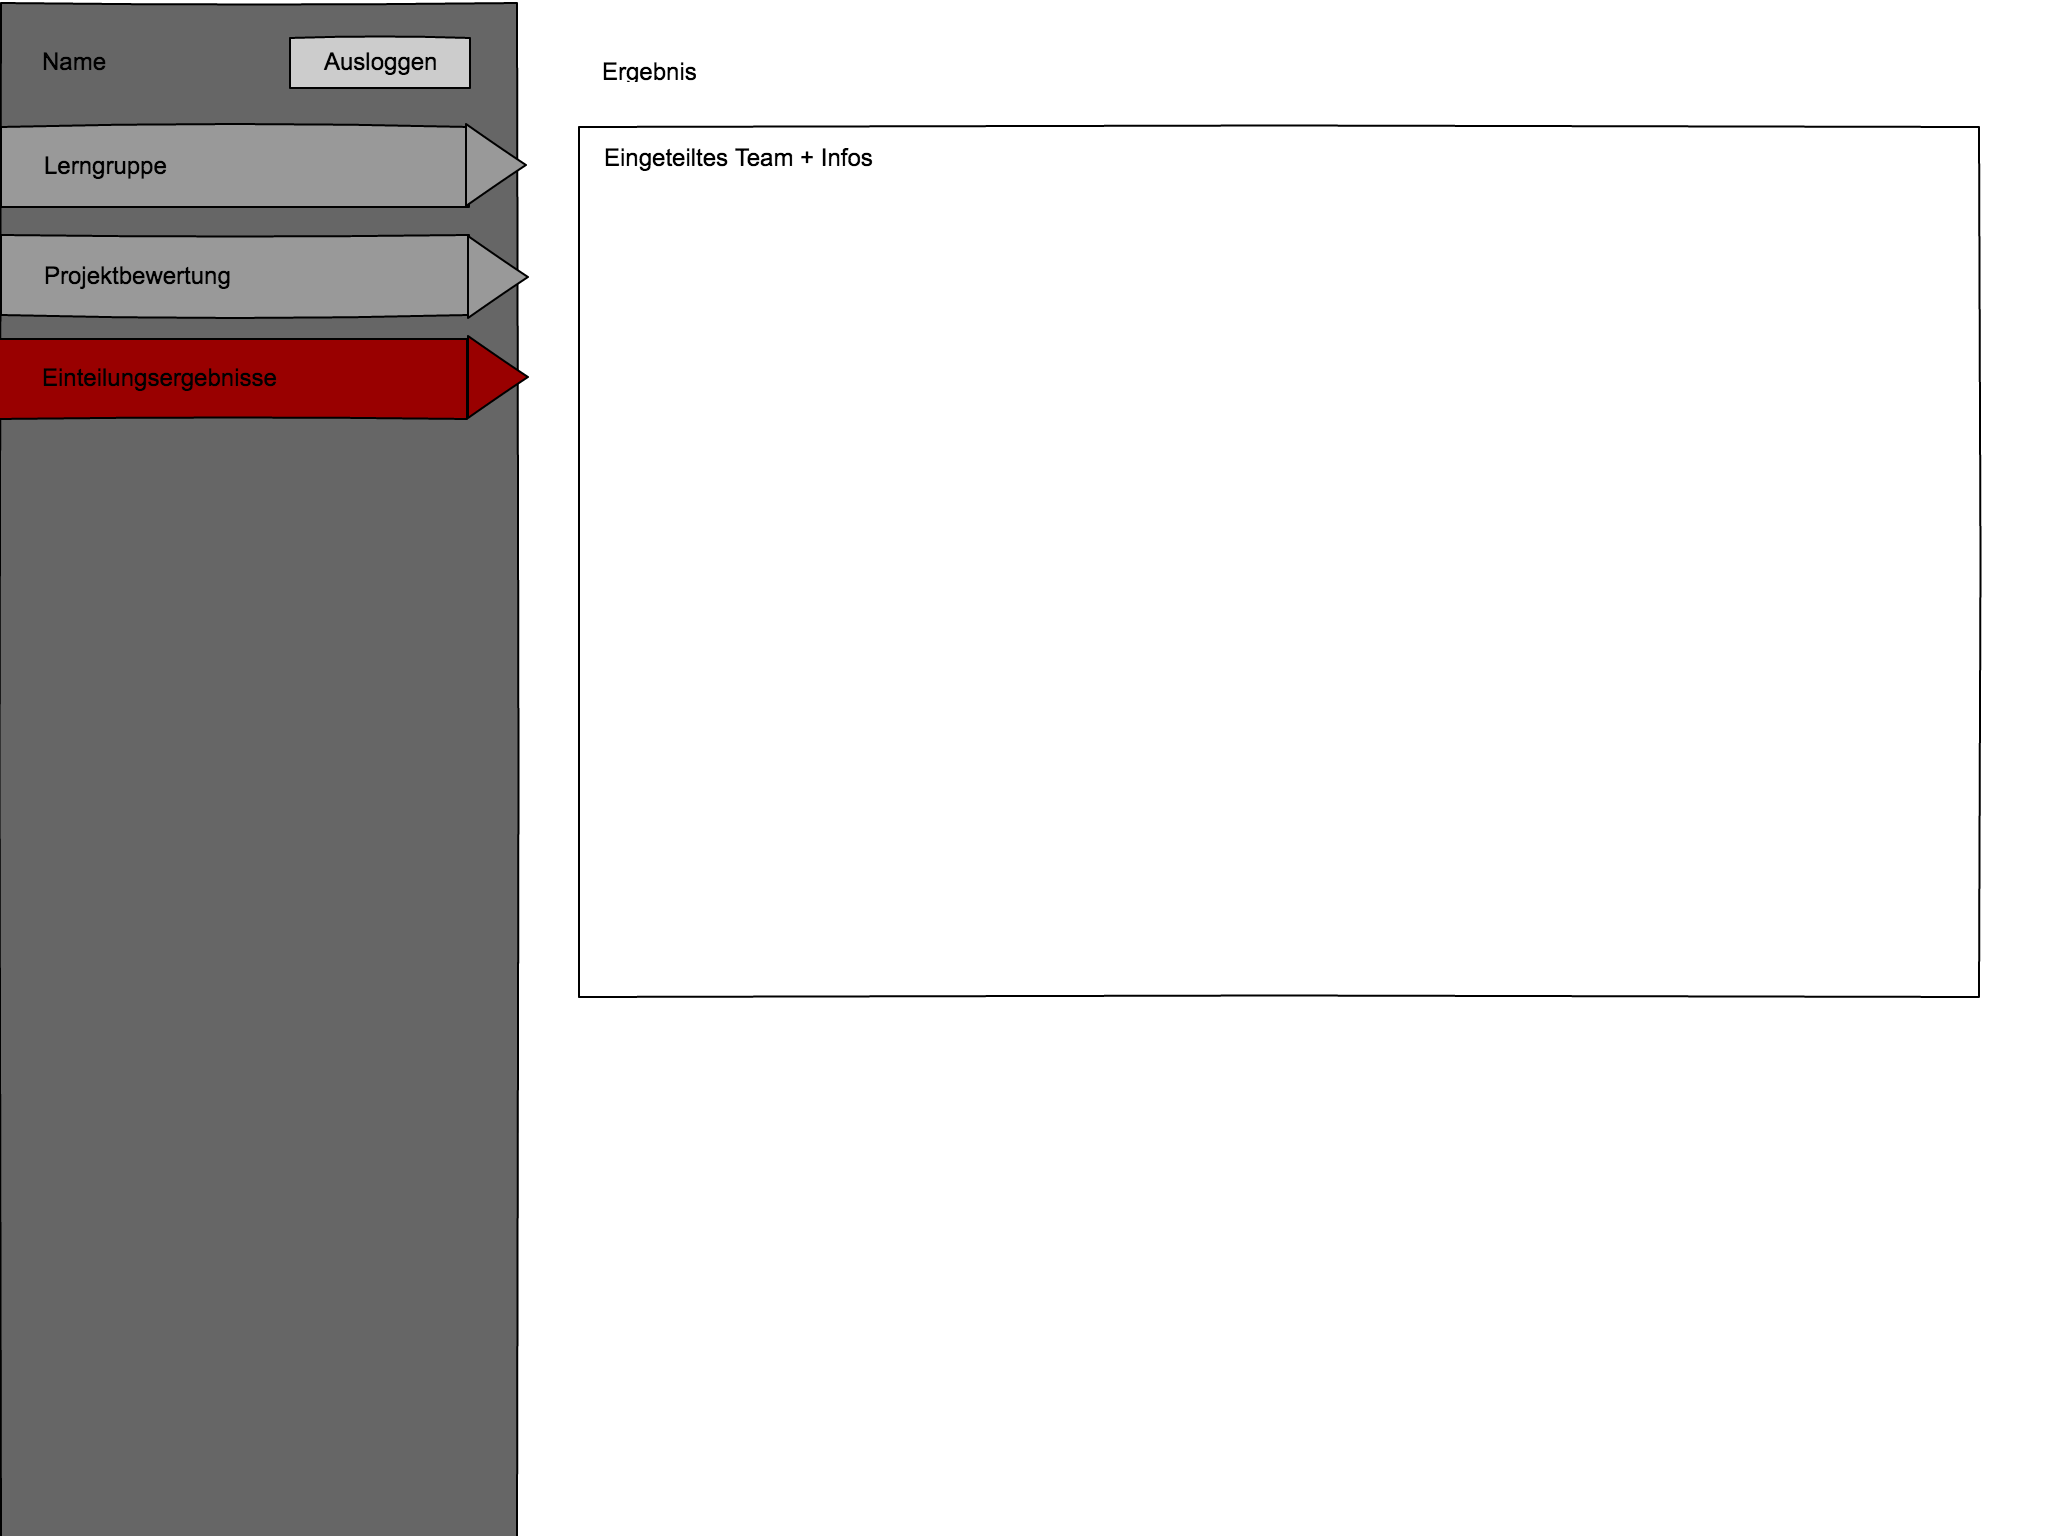
\includegraphics[width=\textwidth,
keepaspectratio=true]{gui/studentergebnis.png}}
\captionof{figure}{Ergebnisansicht}
\medskip
\fbox{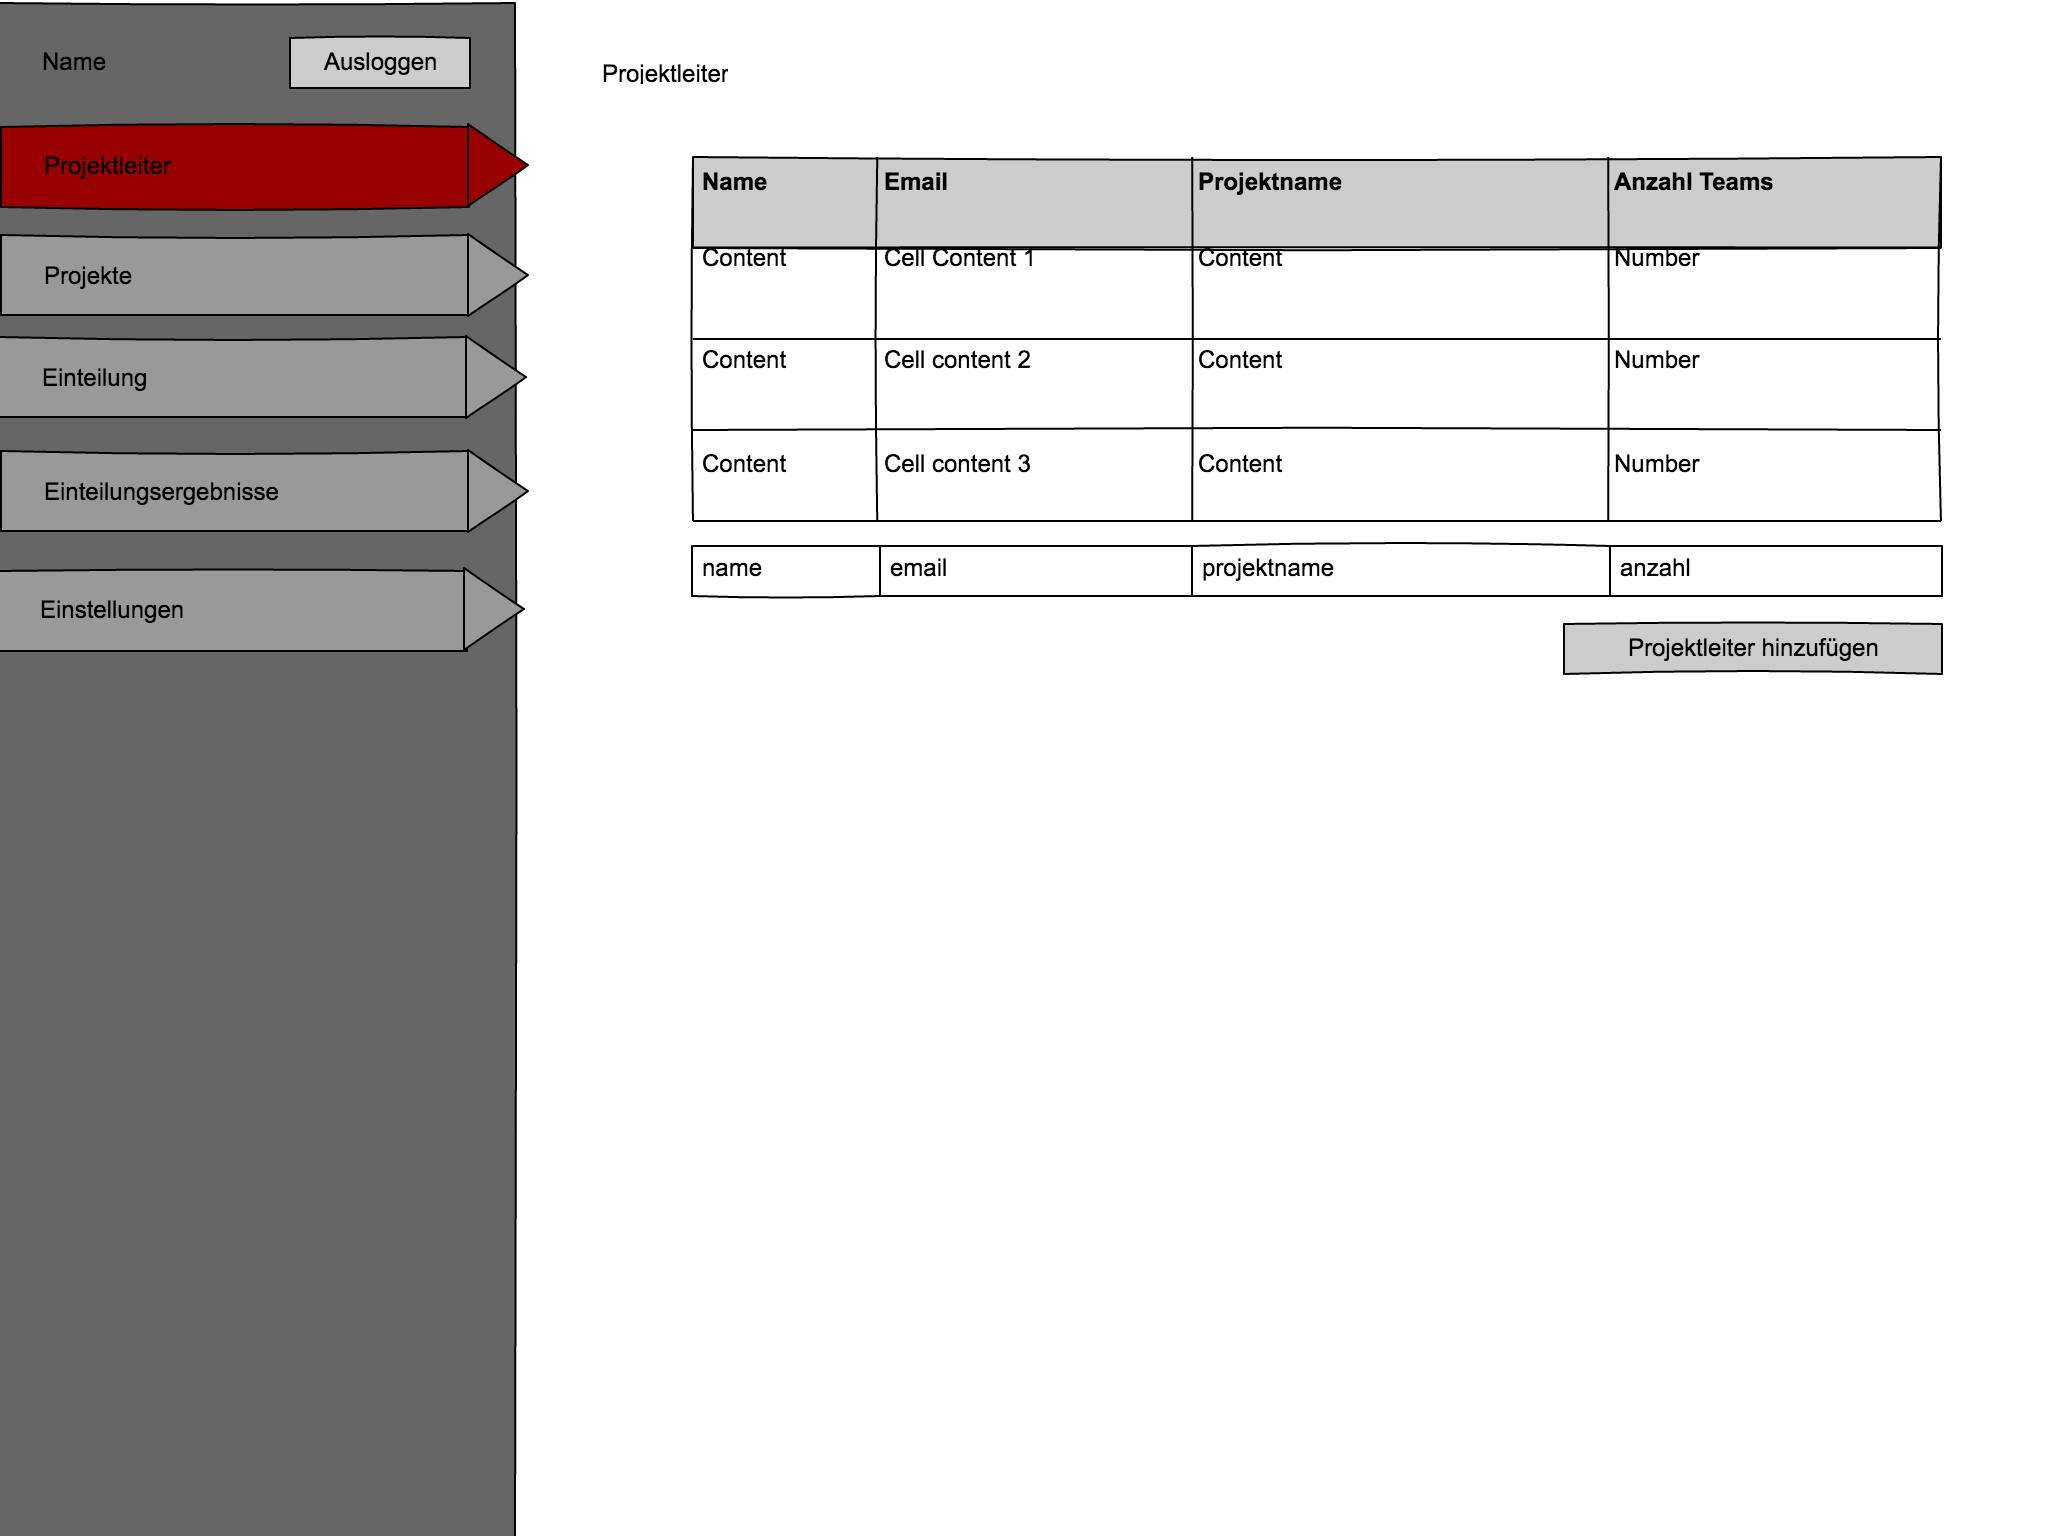
\includegraphics[width=\textwidth,
keepaspectratio=true]{gui/adminprojleiter.png}}
\captionof{figure}{Projektleiterübersicht}
\medskip
\fbox{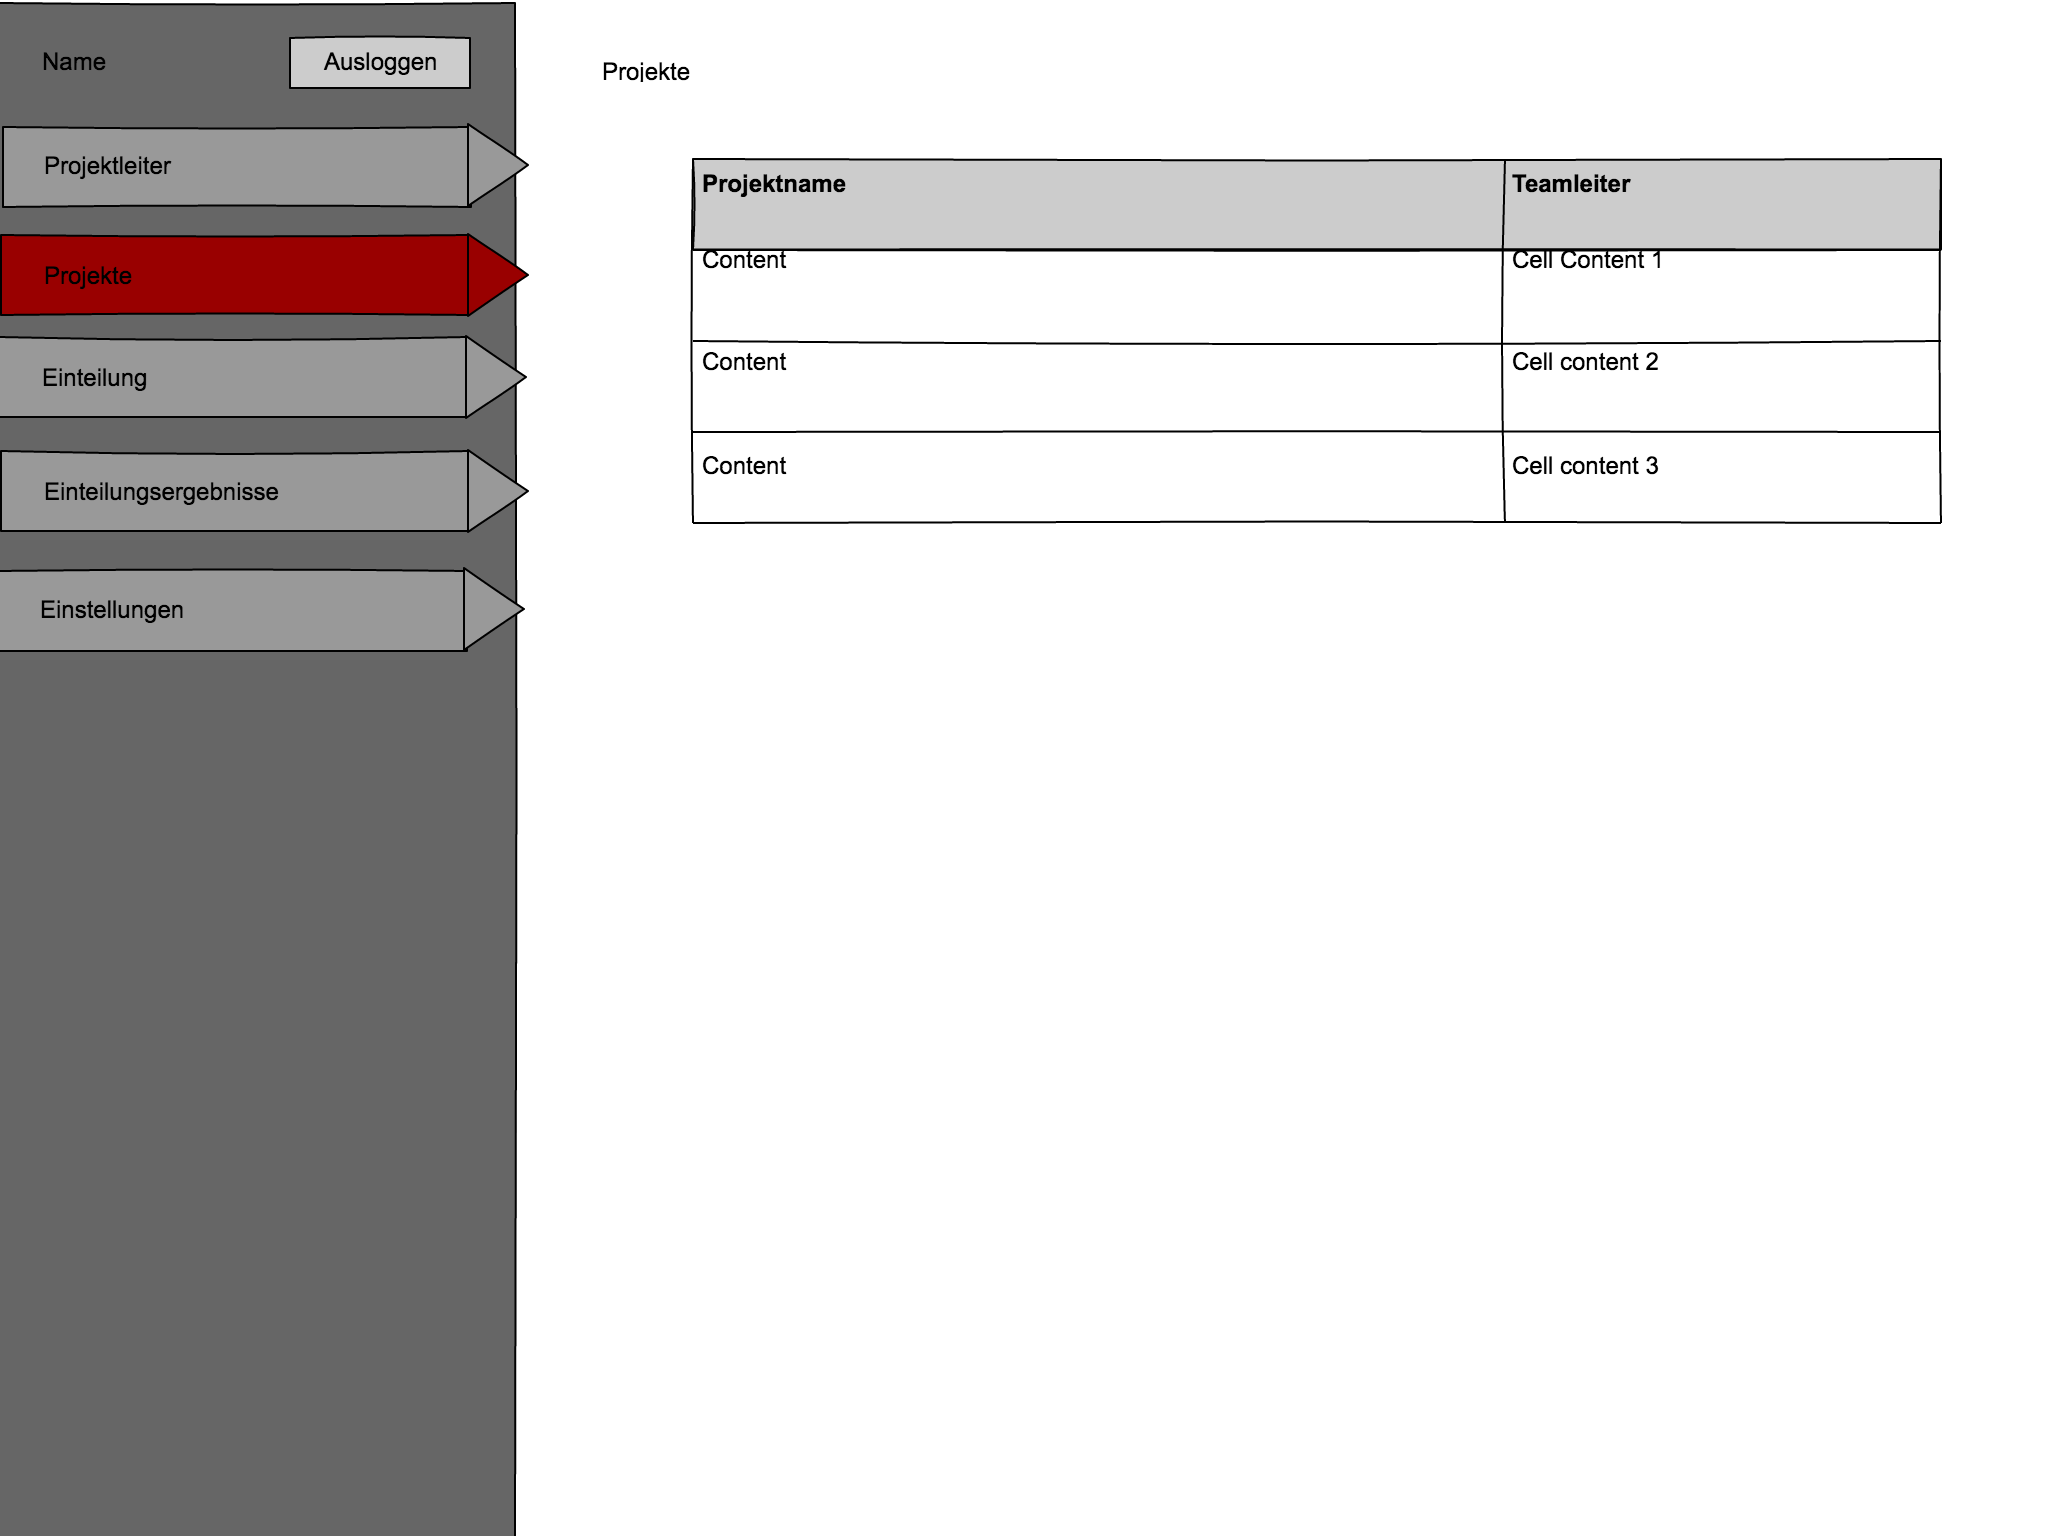
\includegraphics[width=\textwidth,
keepaspectratio=true]{gui/adminprojekte.png}}
\captionof{figure}{Projektübersicht}
\medskip
\fbox{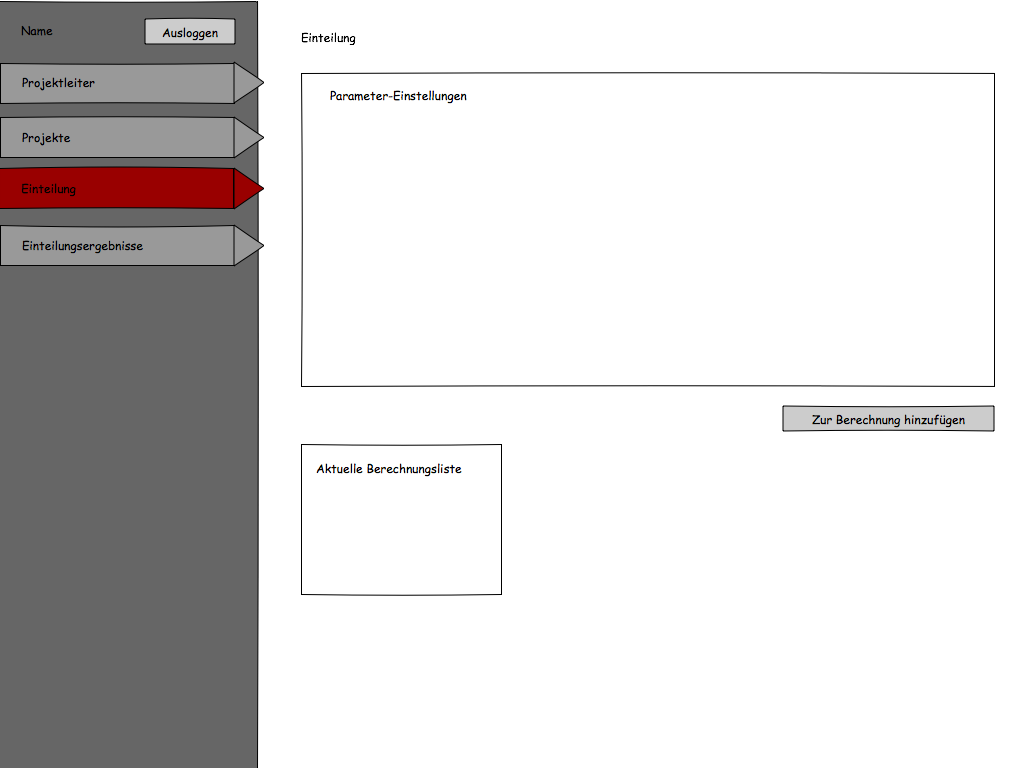
\includegraphics[width=\textwidth,
keepaspectratio=true]{gui/admineinteilung.png}}
\captionof{figure}{Einteilungsmaske}
\medskip
\fbox{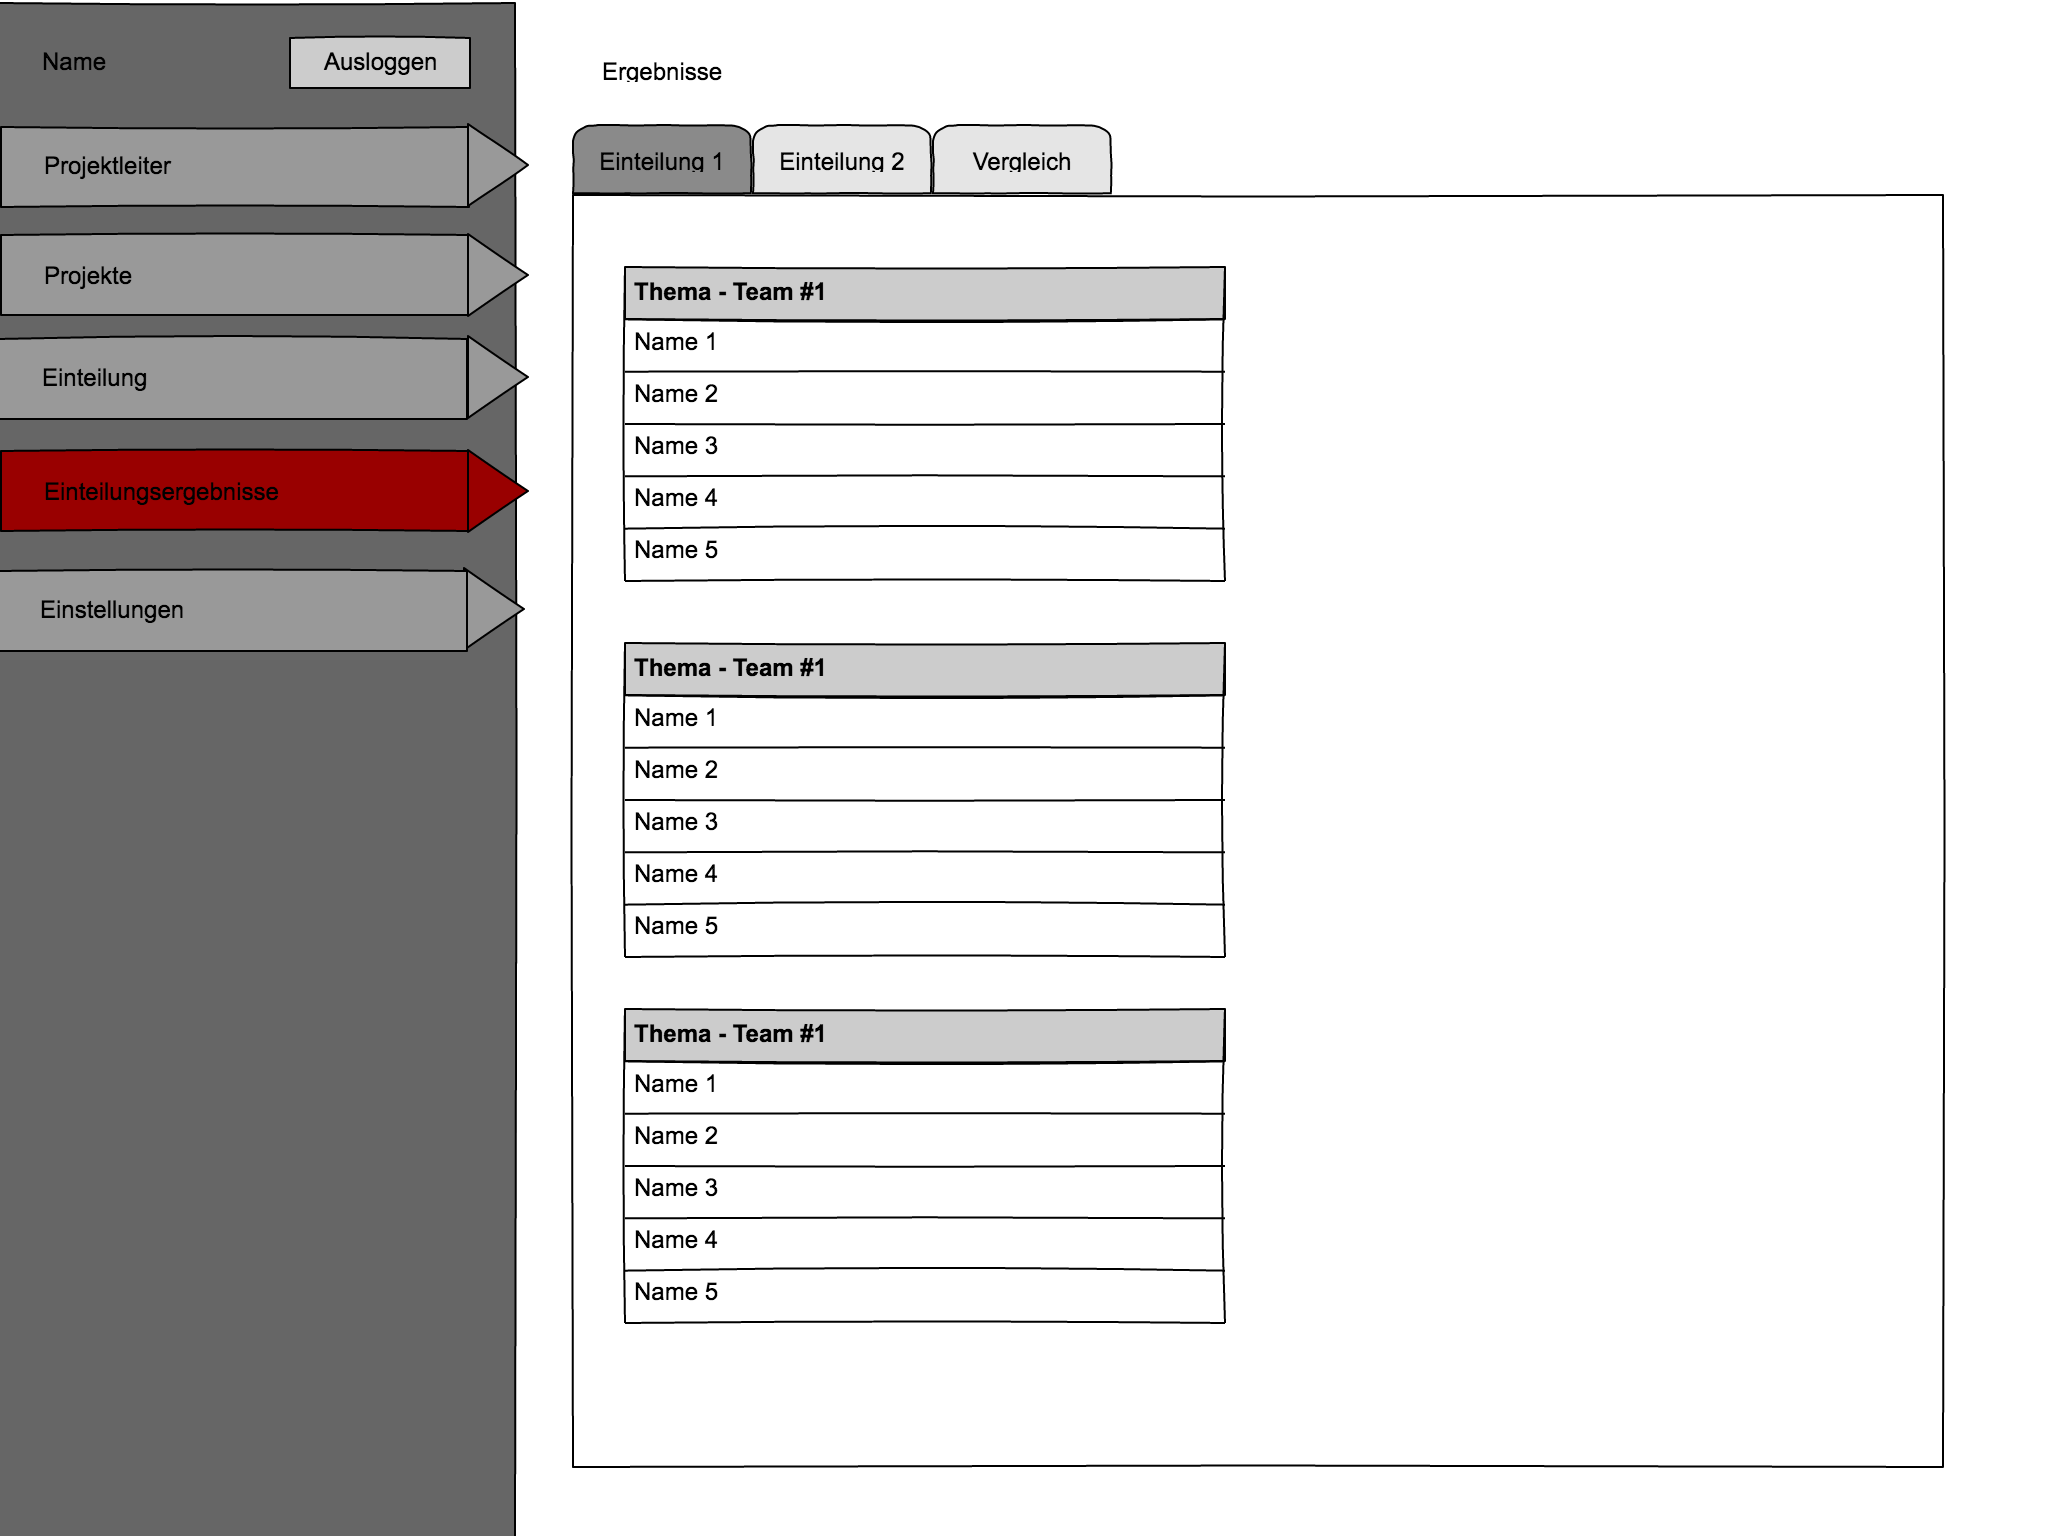
\includegraphics[width=\textwidth,
keepaspectratio=true]{gui/adminergebnisse.png}}
\captionof{figure}{Übersicht der Einteilungen}
\medskip
\fbox{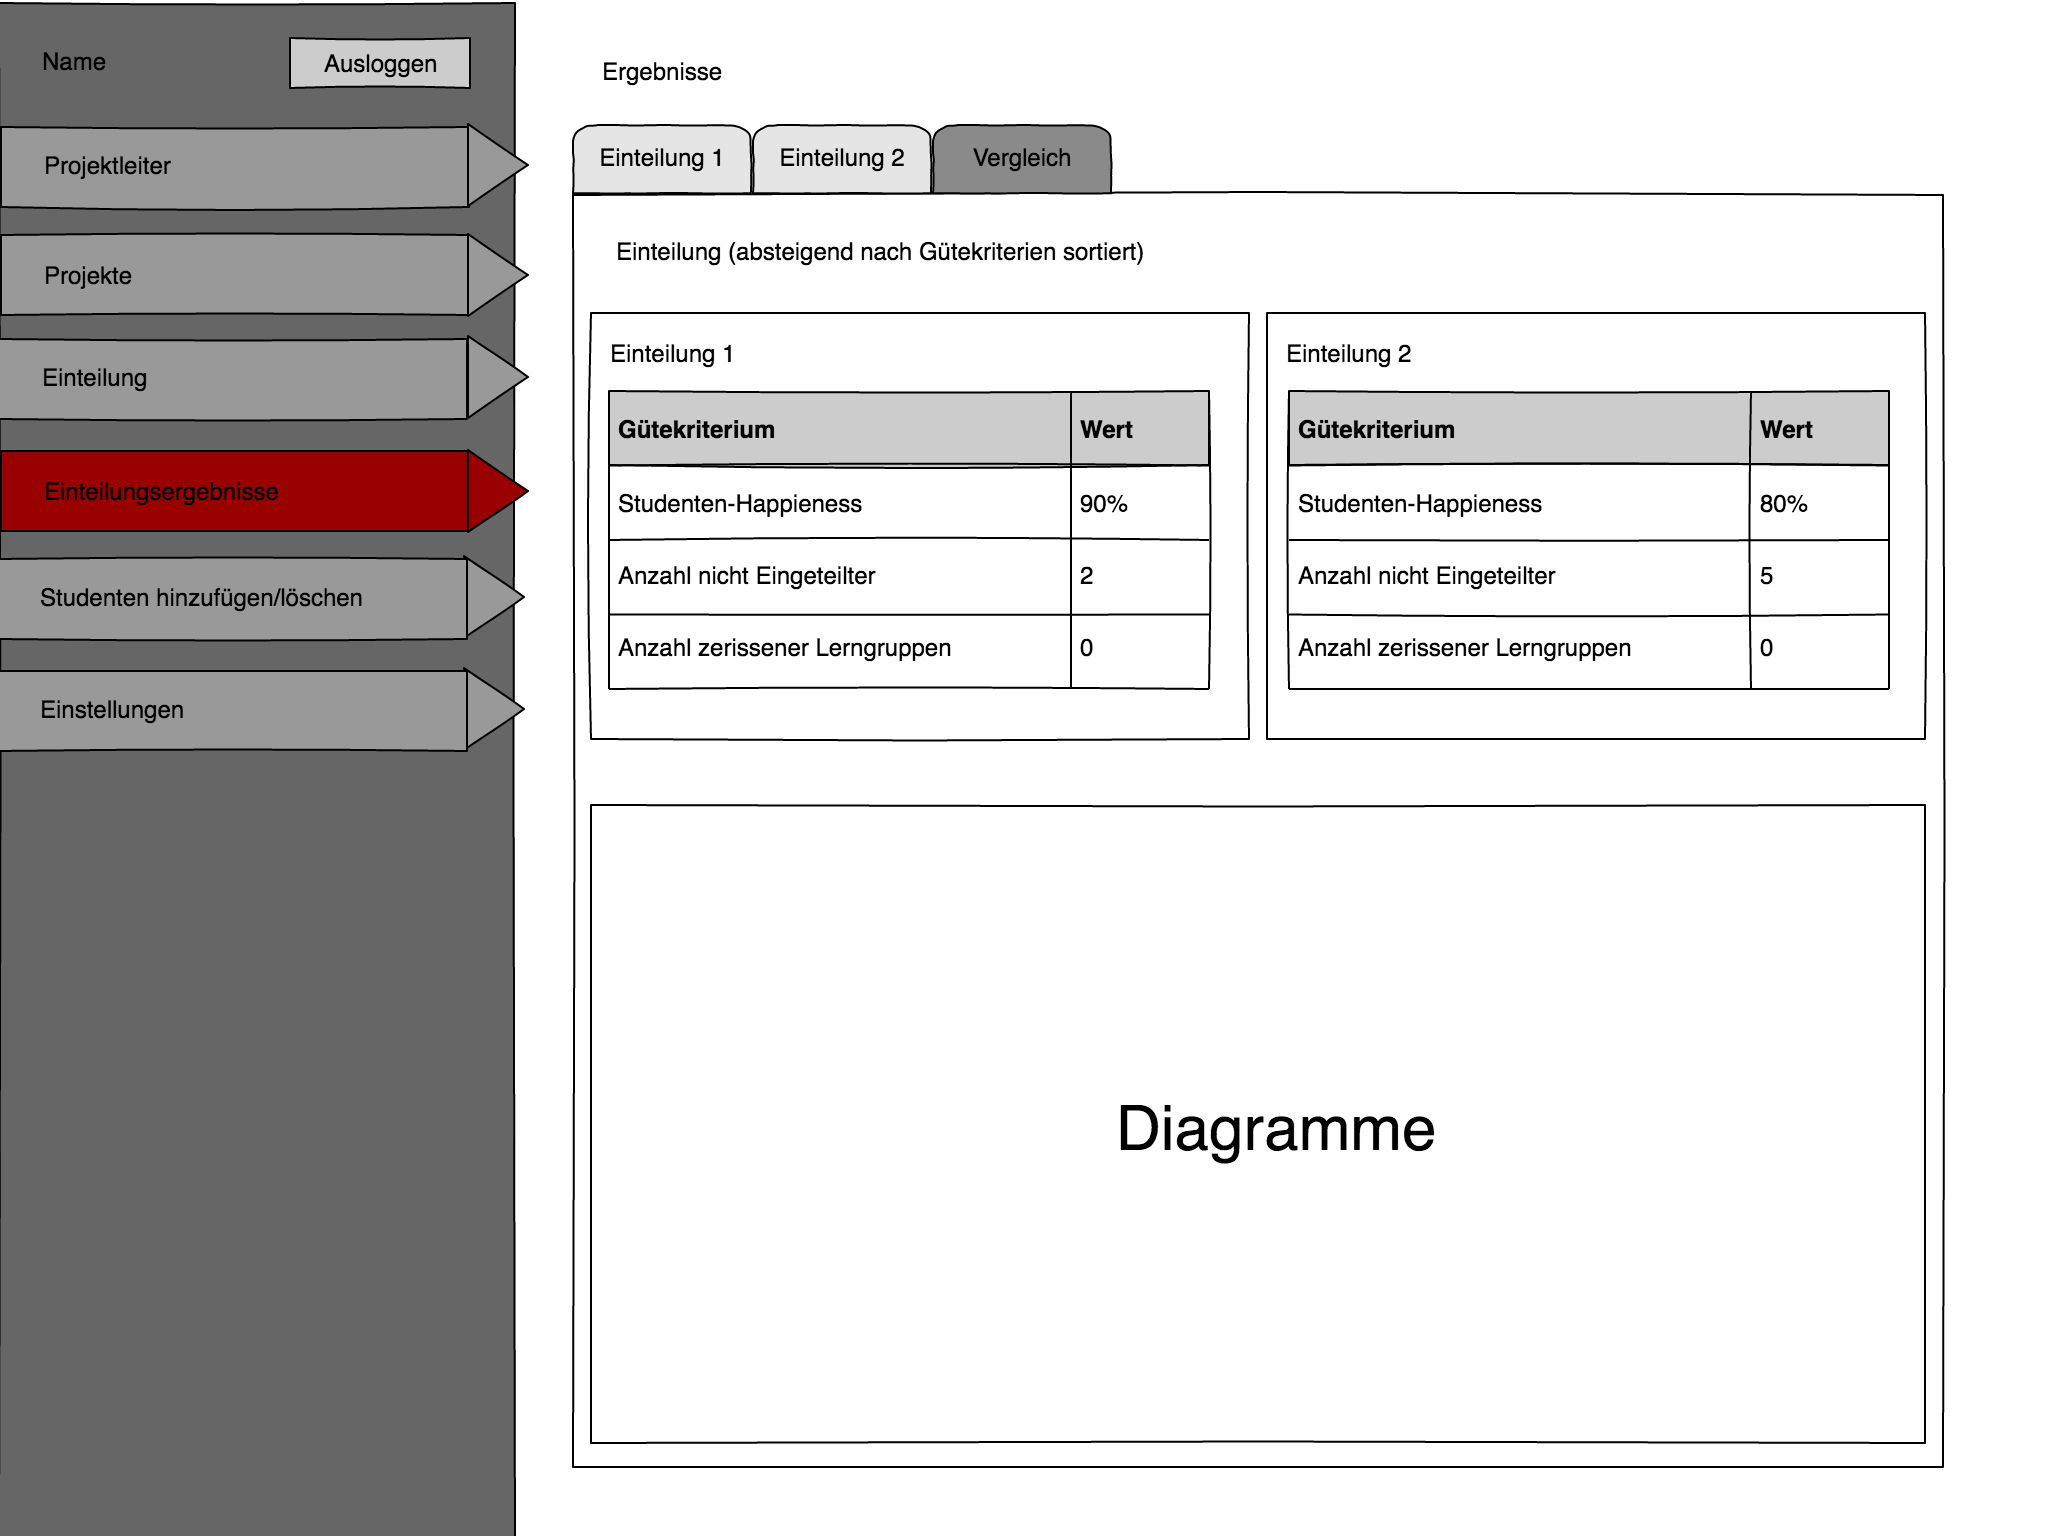
\includegraphics[width=\textwidth,
keepaspectratio=true]{gui/adminergebnissevergl.png}}
\captionof{figure}{Vergleichsansicht}
\medskip
\fbox{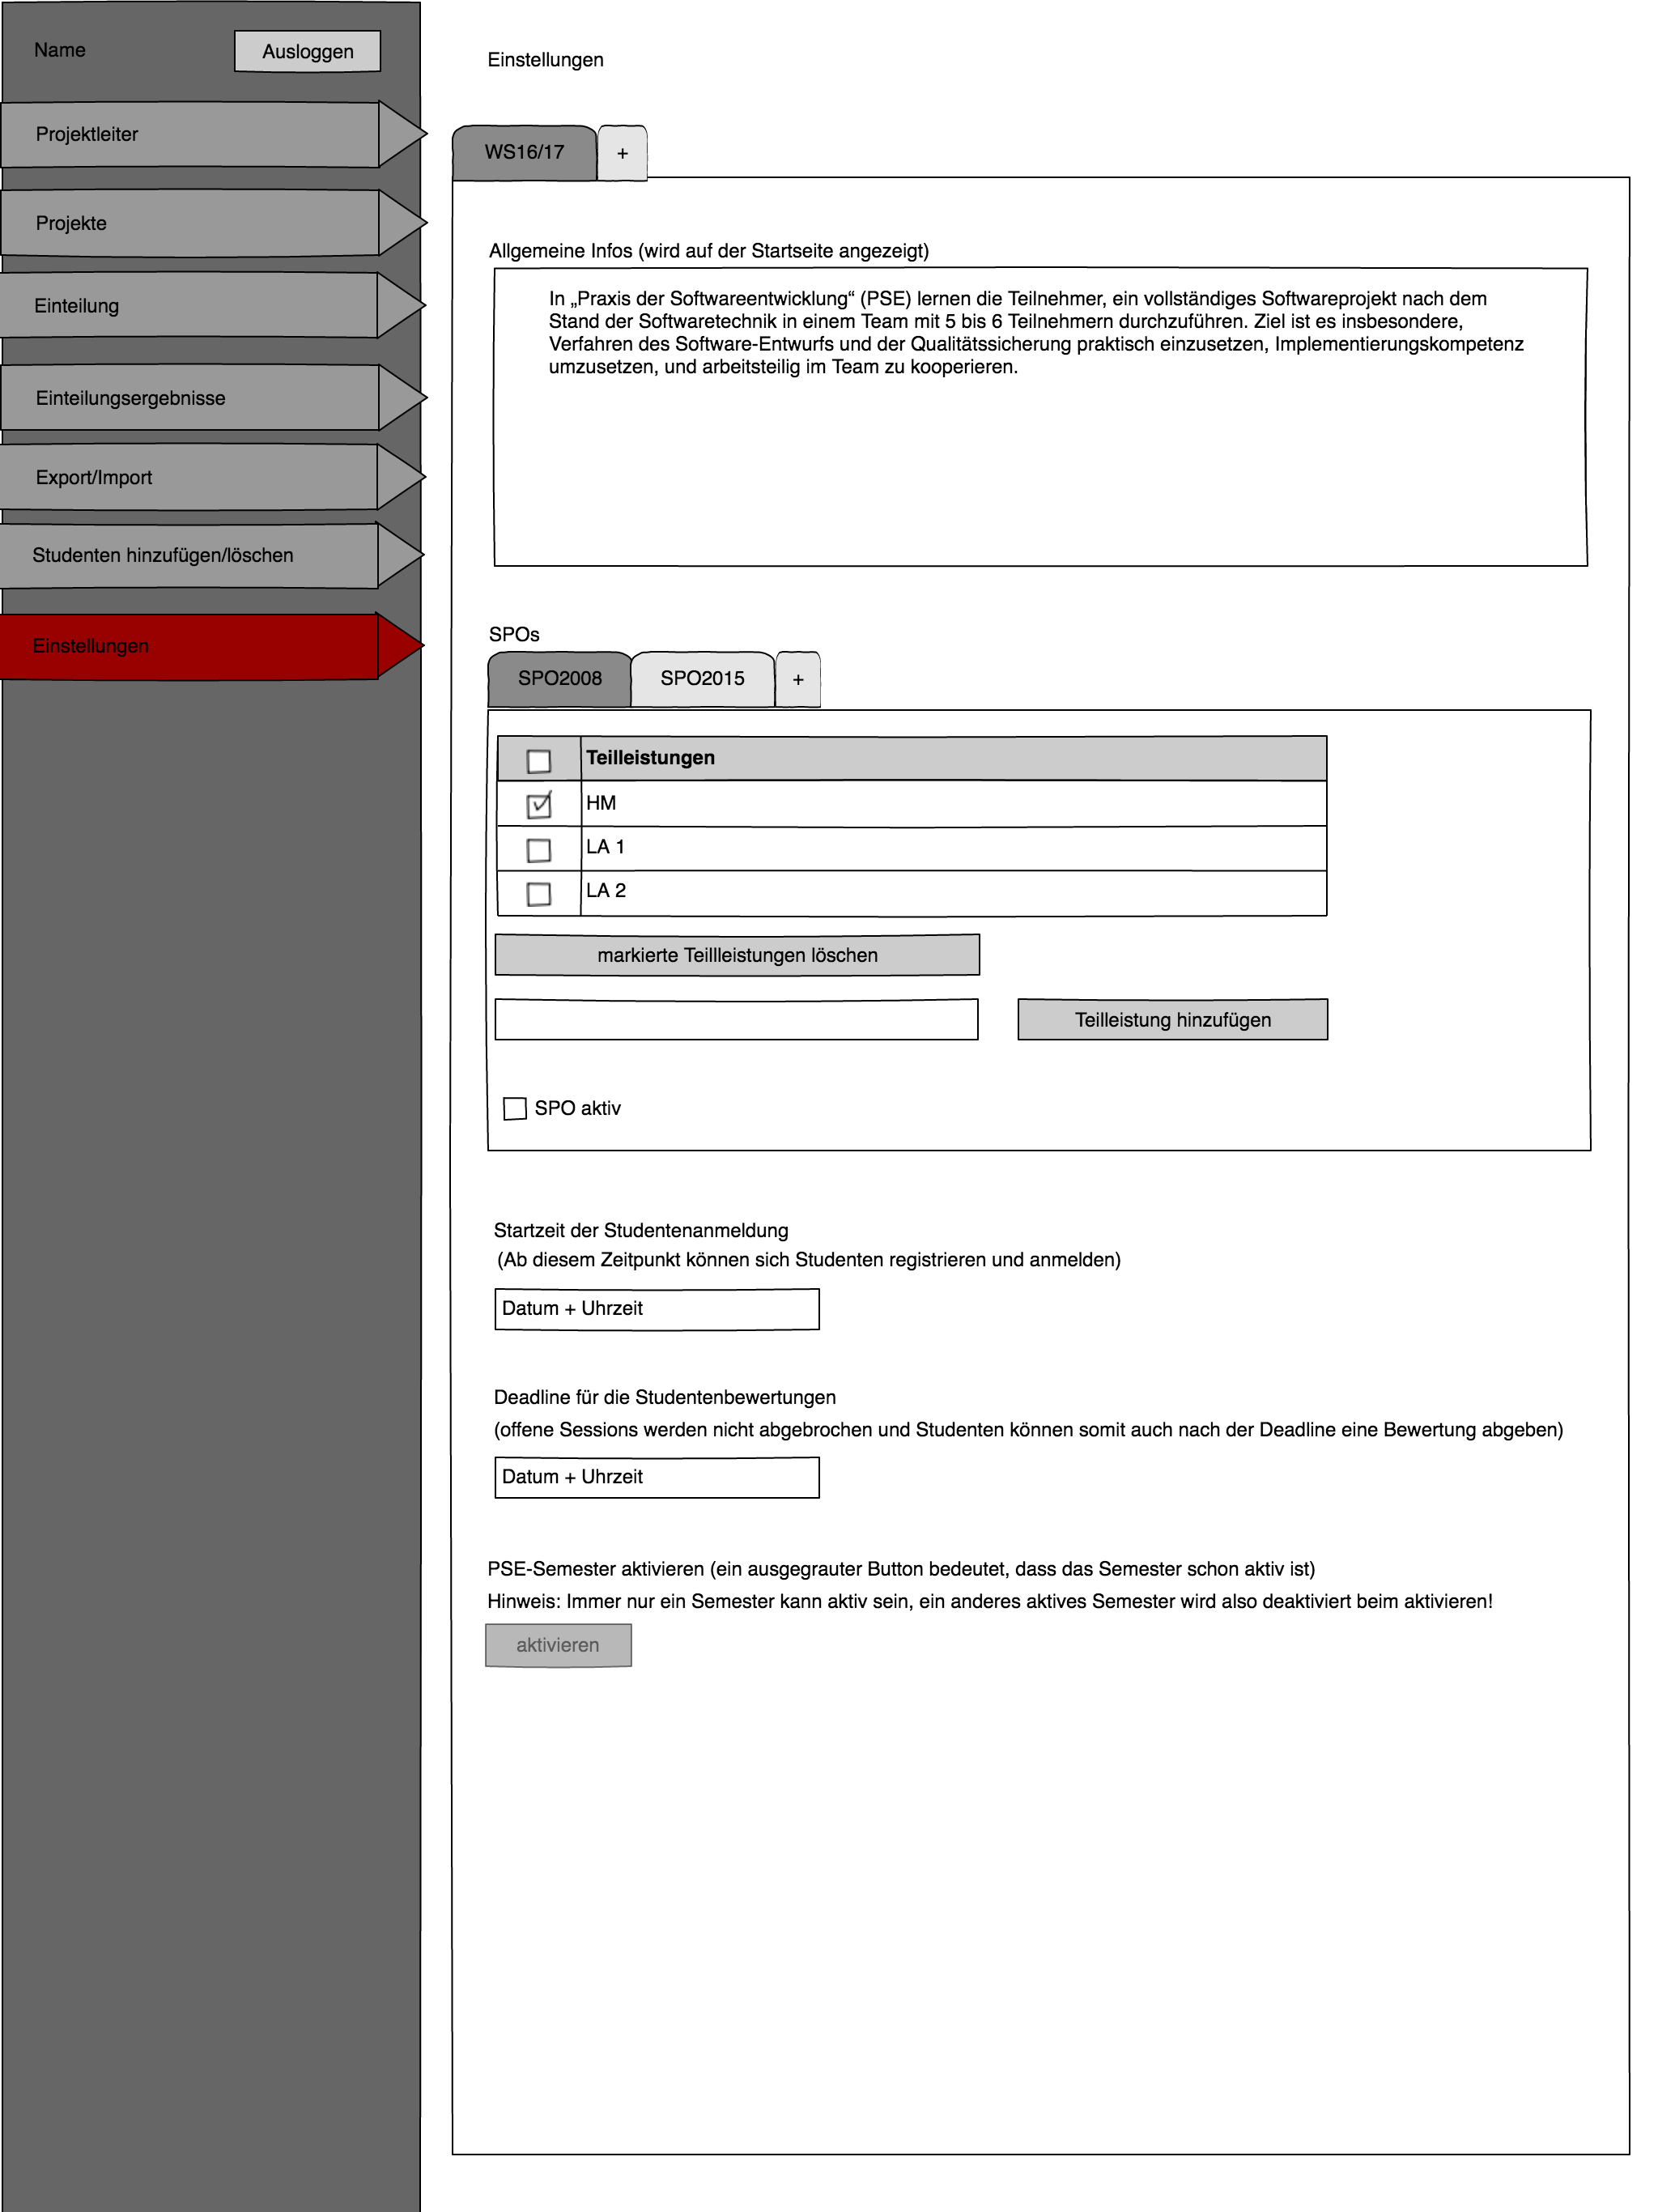
\includegraphics[width=\textwidth,
keepaspectratio=true]{gui/adminproperties.png}}
\captionof{figure}{Einstellungen}
\medskip
\fbox{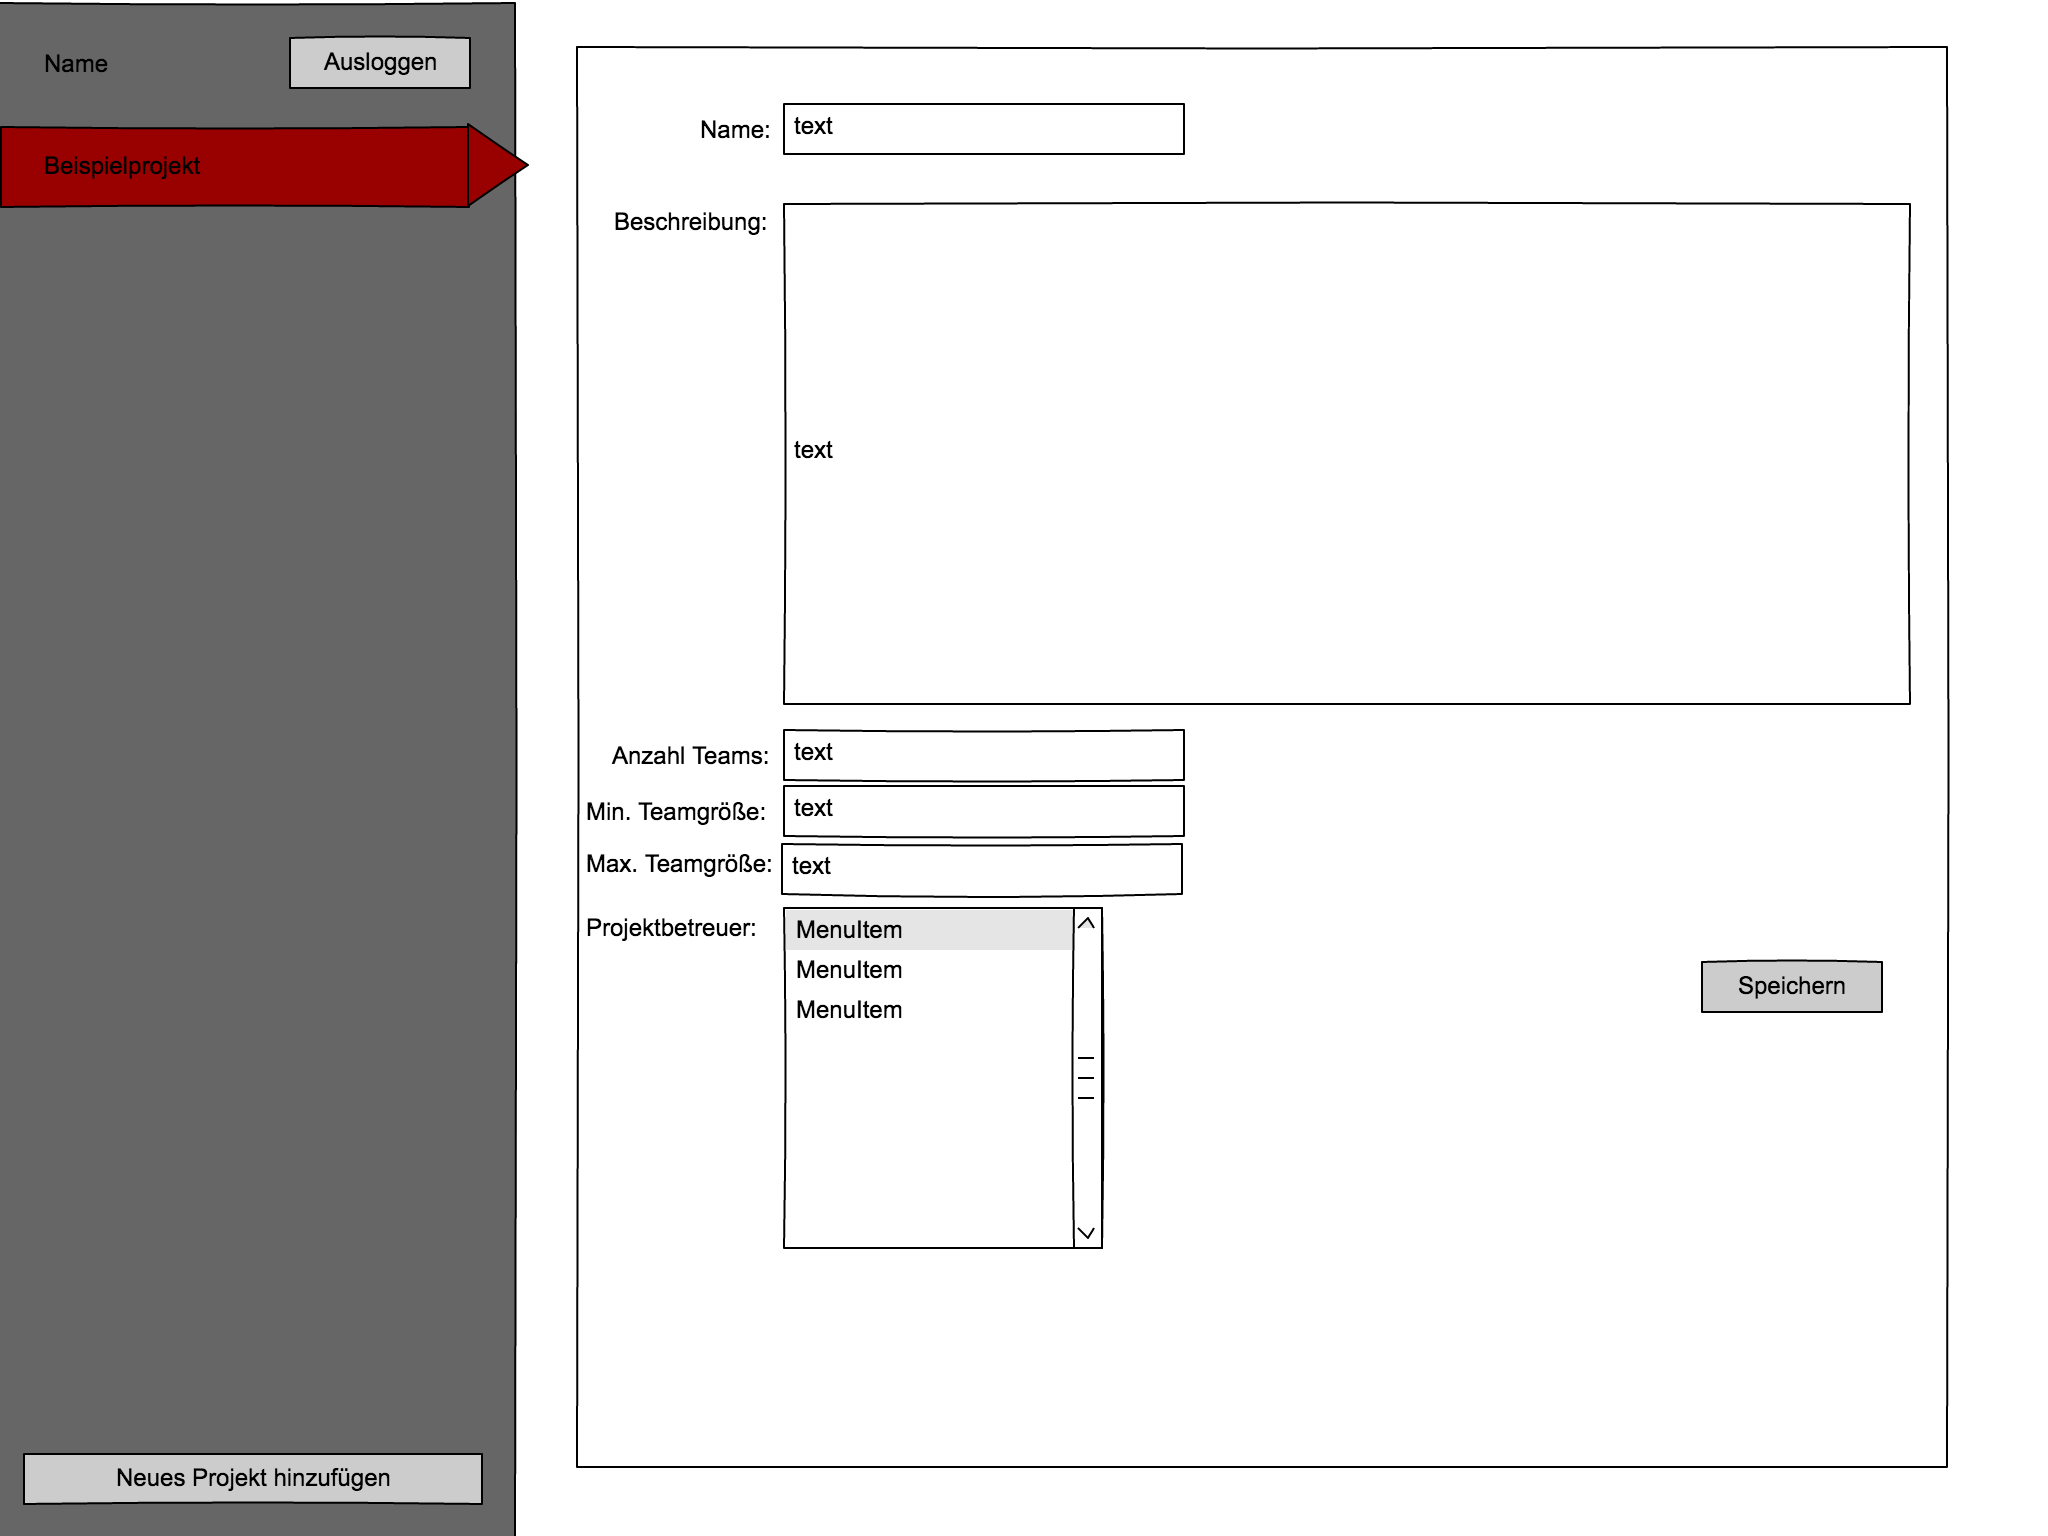
\includegraphics[width=\textwidth,
keepaspectratio=true]{gui/projleiterprojekte.png}}
\captionof{figure}{Betreueransicht}
\medskip
}
\end{enumerate}
\pagebreak
\printglossaries
\end{document}
